\documentclass[10pt]{beamer}

\usetheme[progressbar=frametitle]{metropolis}
\usepackage{appendixnumberbeamer}

\usepackage{booktabs}
\usepackage[scale=2]{ccicons}

\usepackage{pgfplots}
\usepgfplotslibrary{dateplot}

\usepackage{xspace}
\usepackage{comment}
\usepackage{listings}
\usepackage{color}
\usepackage{xcolor}
\newcommand{\themename}{\textbf{\textsc{metropolis}}\xspace}

\newcommand{\cfbox}[2]{%
    \colorlet{currentcolor}{.}%
    {\color{#1}%
    \fbox{\color{currentcolor}#2}}%
}

\title{Apollo}
%\subtitle{A modern beamer theme}
% \date{\today}
\date{}
\author{Matthias Vogelgesang}
\institute{Center for modern beamer themes}
% \titlegraphic{\hfill\includegraphics[height=1.5cm]{logo.pdf}}

\begin{document}

\begin{frame}{}
\vspace*{-0.2cm}
\hspace*{-1.07cm}
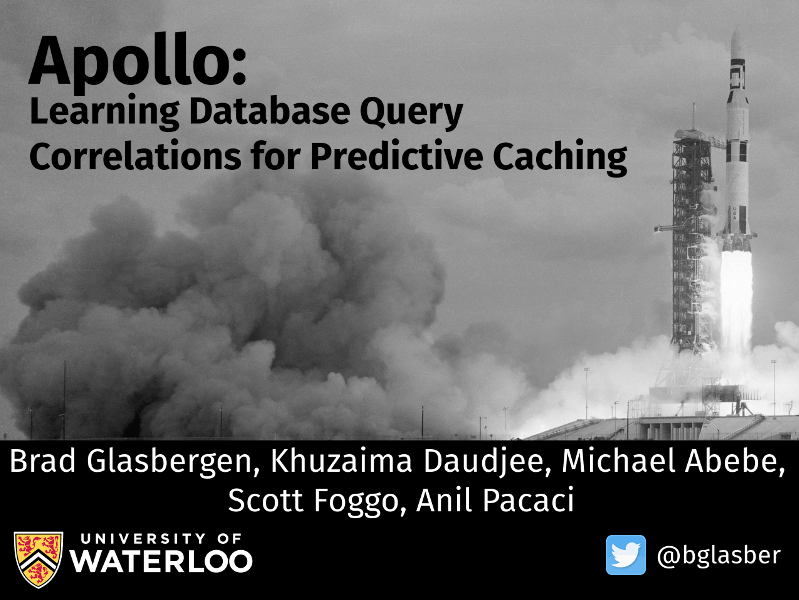
\includegraphics[keepaspectratio=true,width=1.03\paperwidth]{title_slide}
\end{frame}

\begin{frame}{Simple Web Application Architecture}
    \begin{figure}
        \center
        \hspace*{-1cm}
        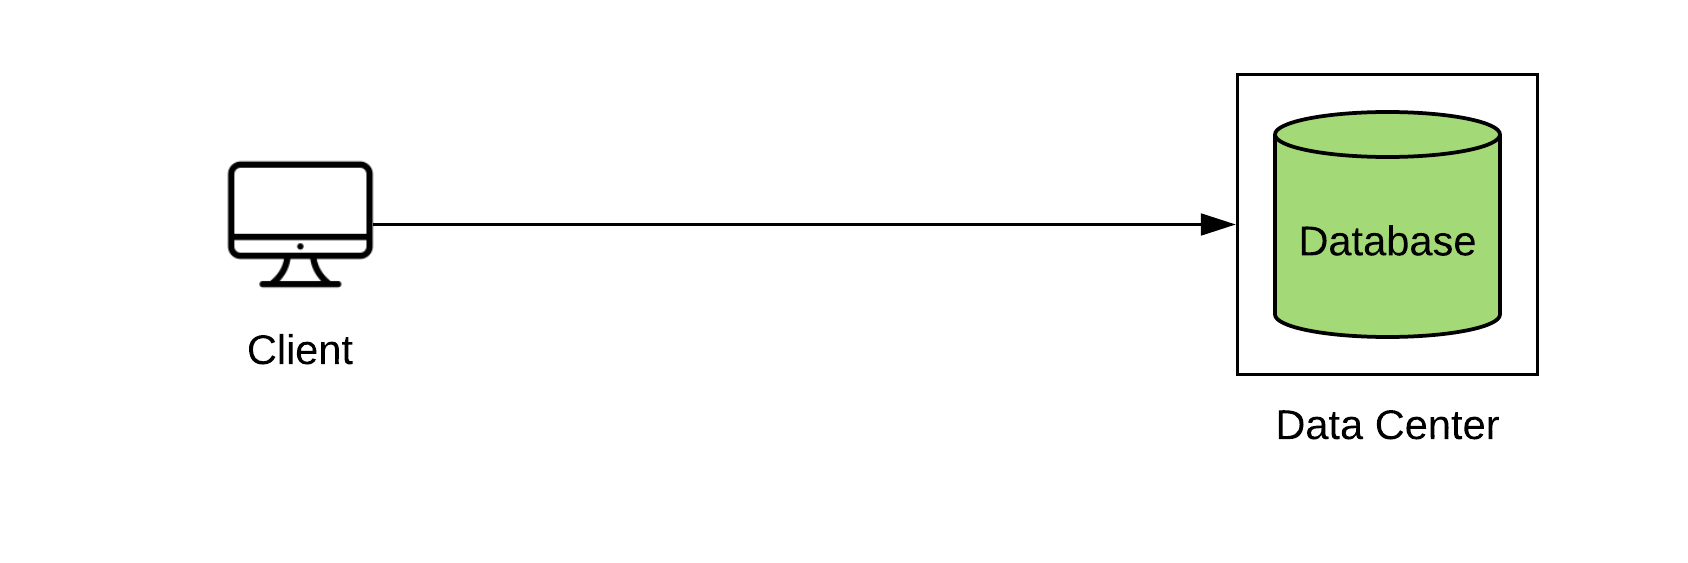
\includegraphics[scale=0.2]{apollo_intro_arch}
    \end{figure}
\end{frame}

\begin{frame}{Worldwide Client/Data Center Distribution}
    \begin{figure}
        \center
        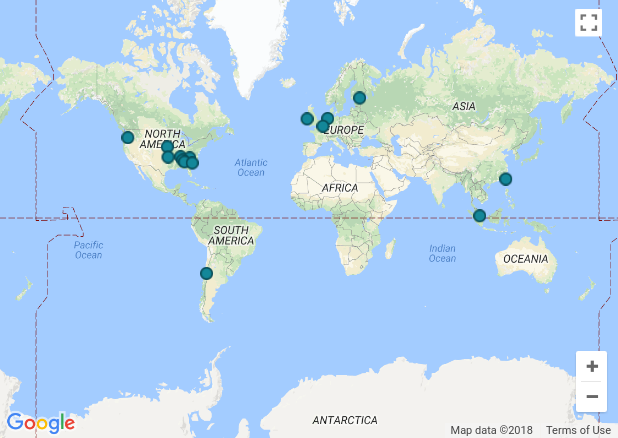
\includegraphics[scale=0.45]{apollo_google_dc}
    \end{figure}
\end{frame}

\begin{frame}{Worldwide Client/Data Center Distribution}
    \begin{figure}
        \center
        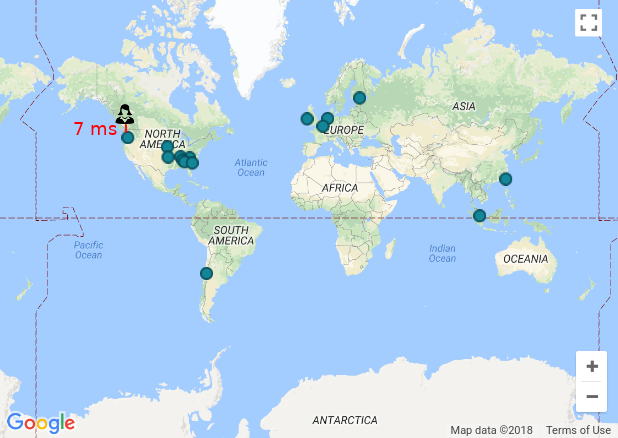
\includegraphics[scale=0.45]{apollo_google_vancouver}
    \end{figure}
\end{frame}

\begin{frame}{Worldwide Client/Data Center Distribution}
    \begin{figure}
        \center
        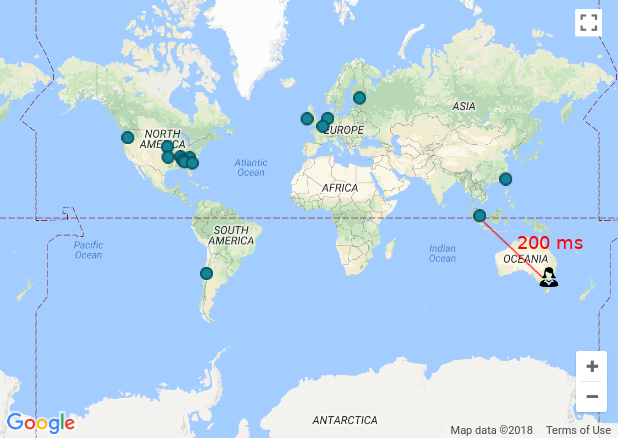
\includegraphics[scale=0.45]{apollo_google_oceania}
    \end{figure}
\end{frame}

\begin{frame}{Latency Effects on Clients}
    Increased latency reduces \alert{user engagement}, and consequently \alert{revenue}! \\
    \vspace{1cm}

    \small{Schurman et al., ``Performance Related Changes and Their User Impact''. \emph{Velocity}, 2009.}
\end{frame}

\begin{frame}{Edge Caching (Content Delivery Networks)}
    \begin{figure}
        \center
        \hspace*{-1.5cm}
        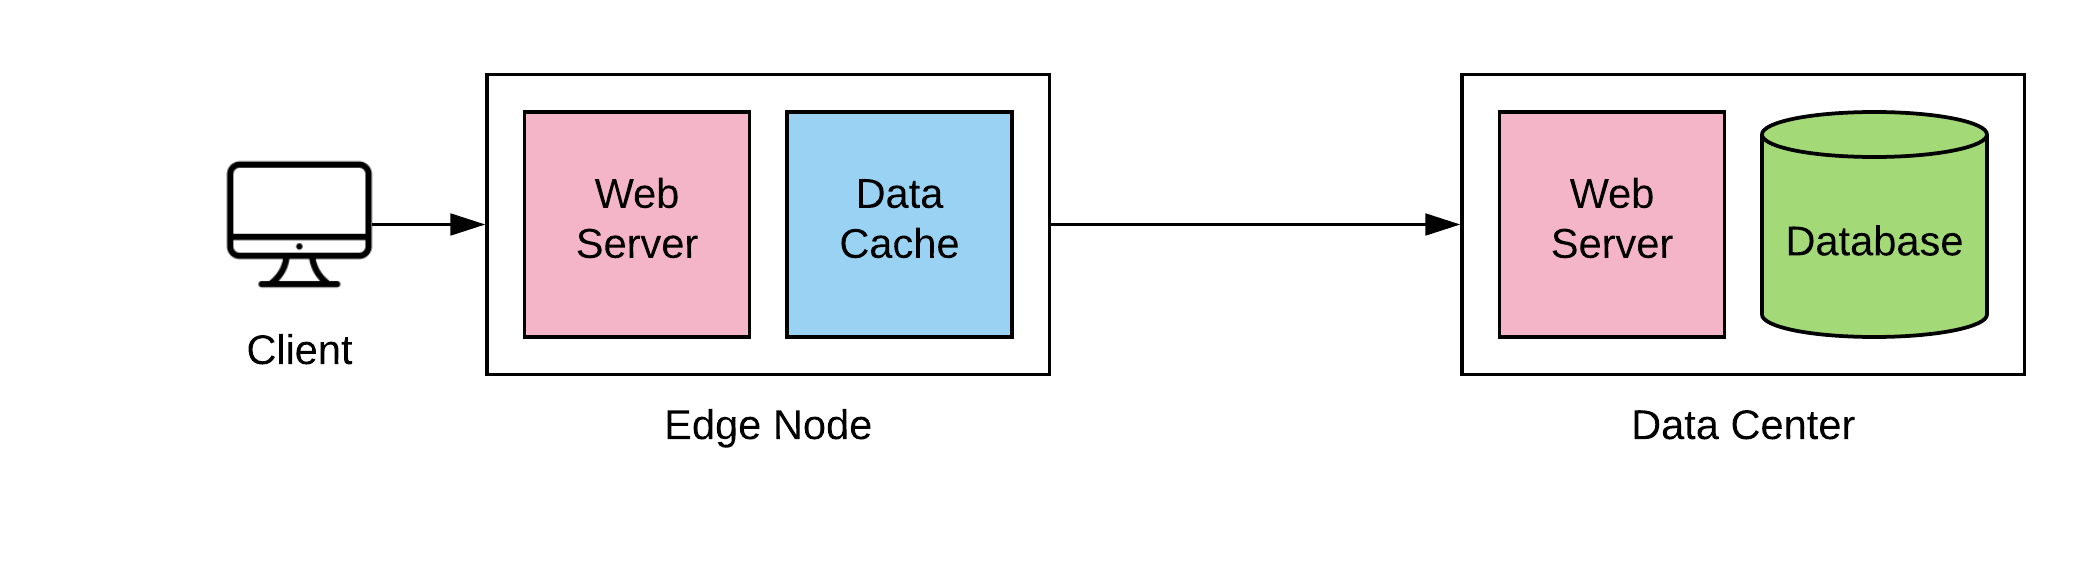
\includegraphics[scale=0.17]{apollo_edge_cache}
    \end{figure}
\end{frame}

\begin{frame}{Worldwide Client/Edge Node Distribution}
    \begin{figure}
        \center
        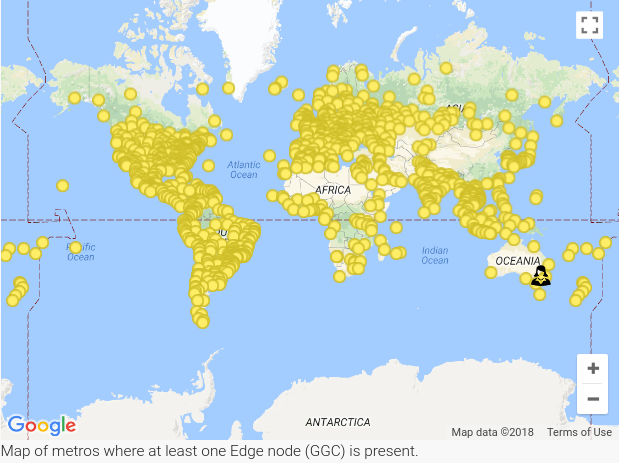
\includegraphics[scale=0.45]{apollo_google_oceania_en}
    \end{figure}
\end{frame}

\begin{frame}{A Problem}
    \begin{itemize}
        \item{Existing edge caches support only \alert{static data}!}
        \visible<2->{
            \item{A majority of webpages rely on personalization and changing data!}
        }
    \end{itemize}
    \vspace{1cm}
    \visible<2->{
    \small{Amiri et al., ``DBProxy: a dynamic data cache for web applications,'' \emph{ICDE}, 2003.}
}
\end{frame}

\begin{frame}{Static Data Edge Cache Architecture}
    \begin{figure}
        \center
        \hspace*{-1.5cm}
        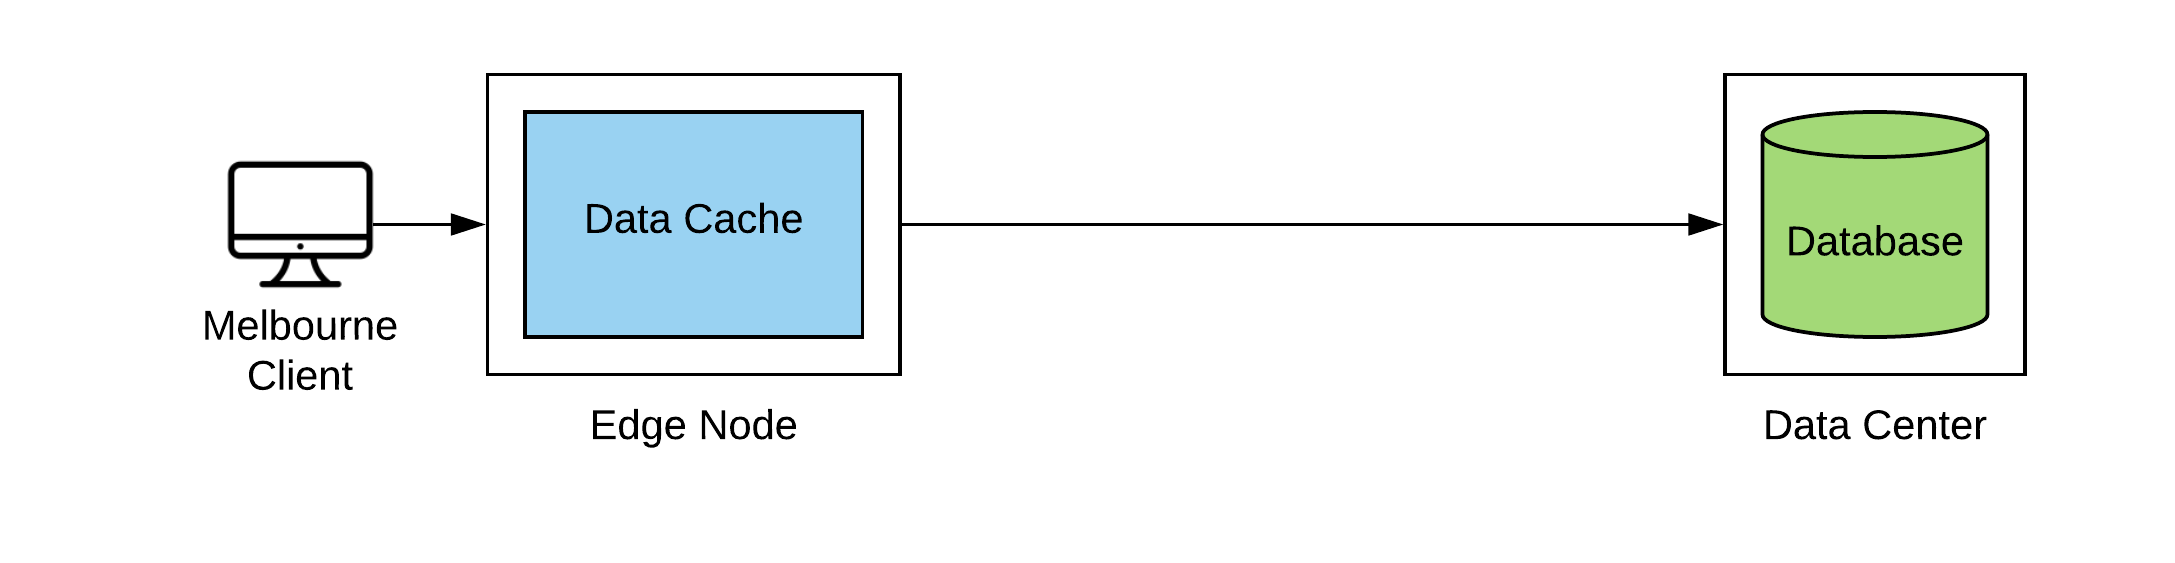
\includegraphics[scale=0.17]{apollo_ec_dbl_0}
    \end{figure}
\end{frame}

\begin{frame}{Extending Edge Cache Support}
    \begin{figure}
        \center
        \hspace*{-1.5cm}
        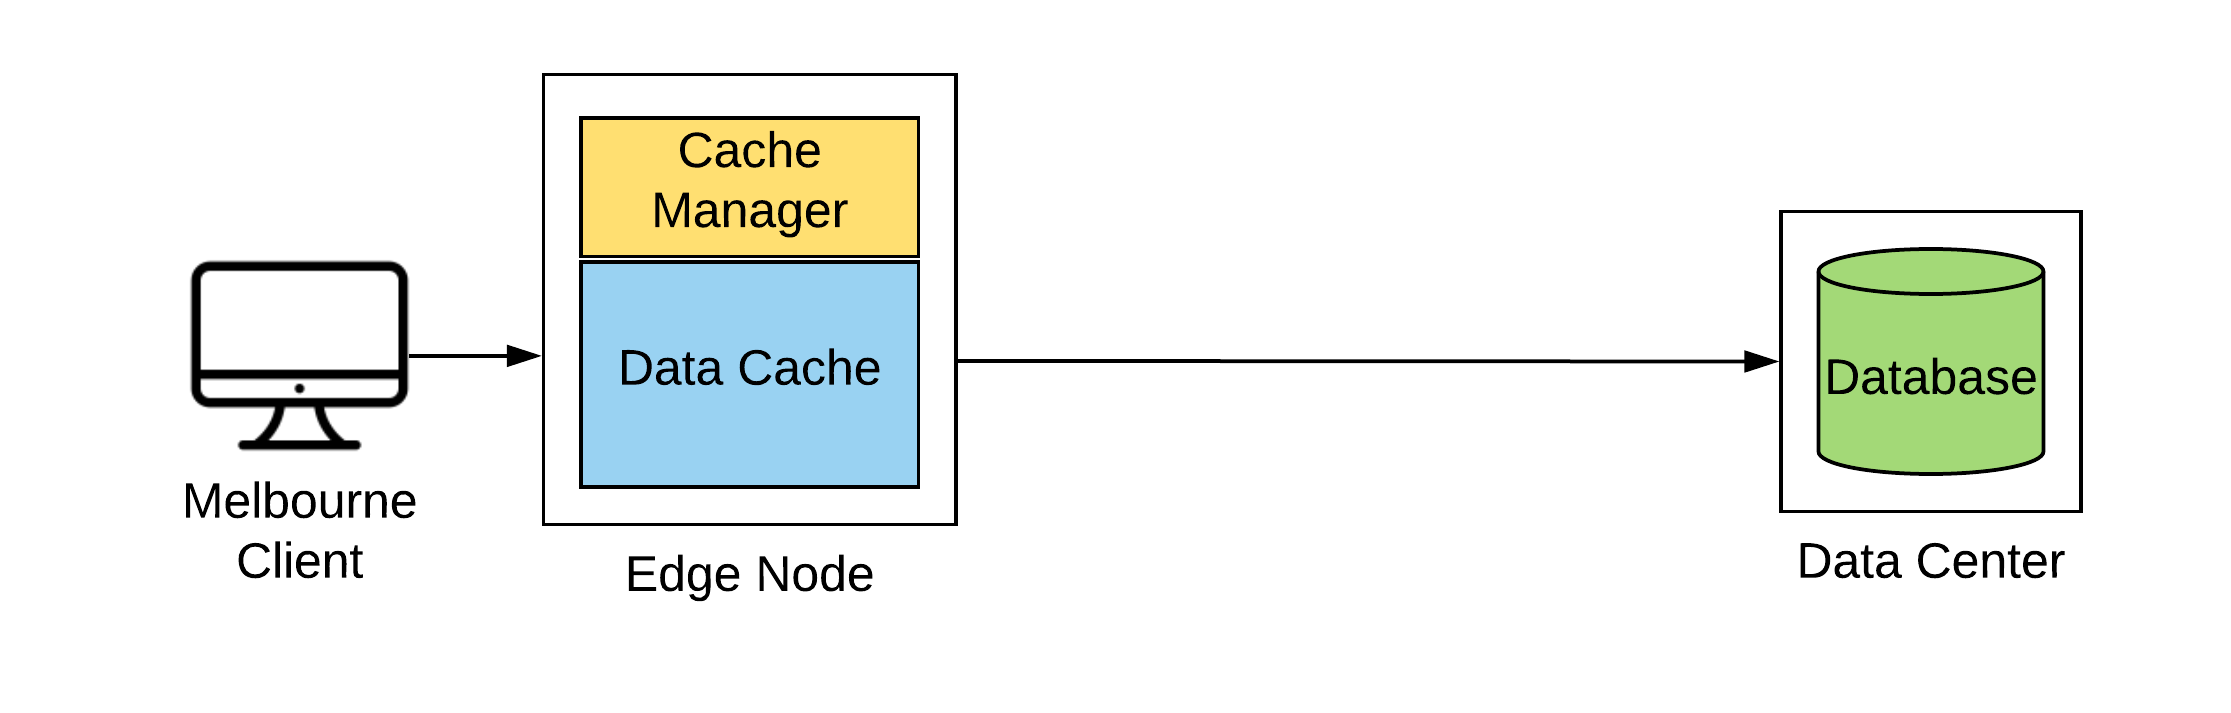
\includegraphics[scale=0.17]{apollo_ec_dbl}
    \end{figure}
\end{frame}

\begin{frame}{Extending Edge Cache Support}
    \begin{figure}
        \center
        \hspace*{-1.5cm}
        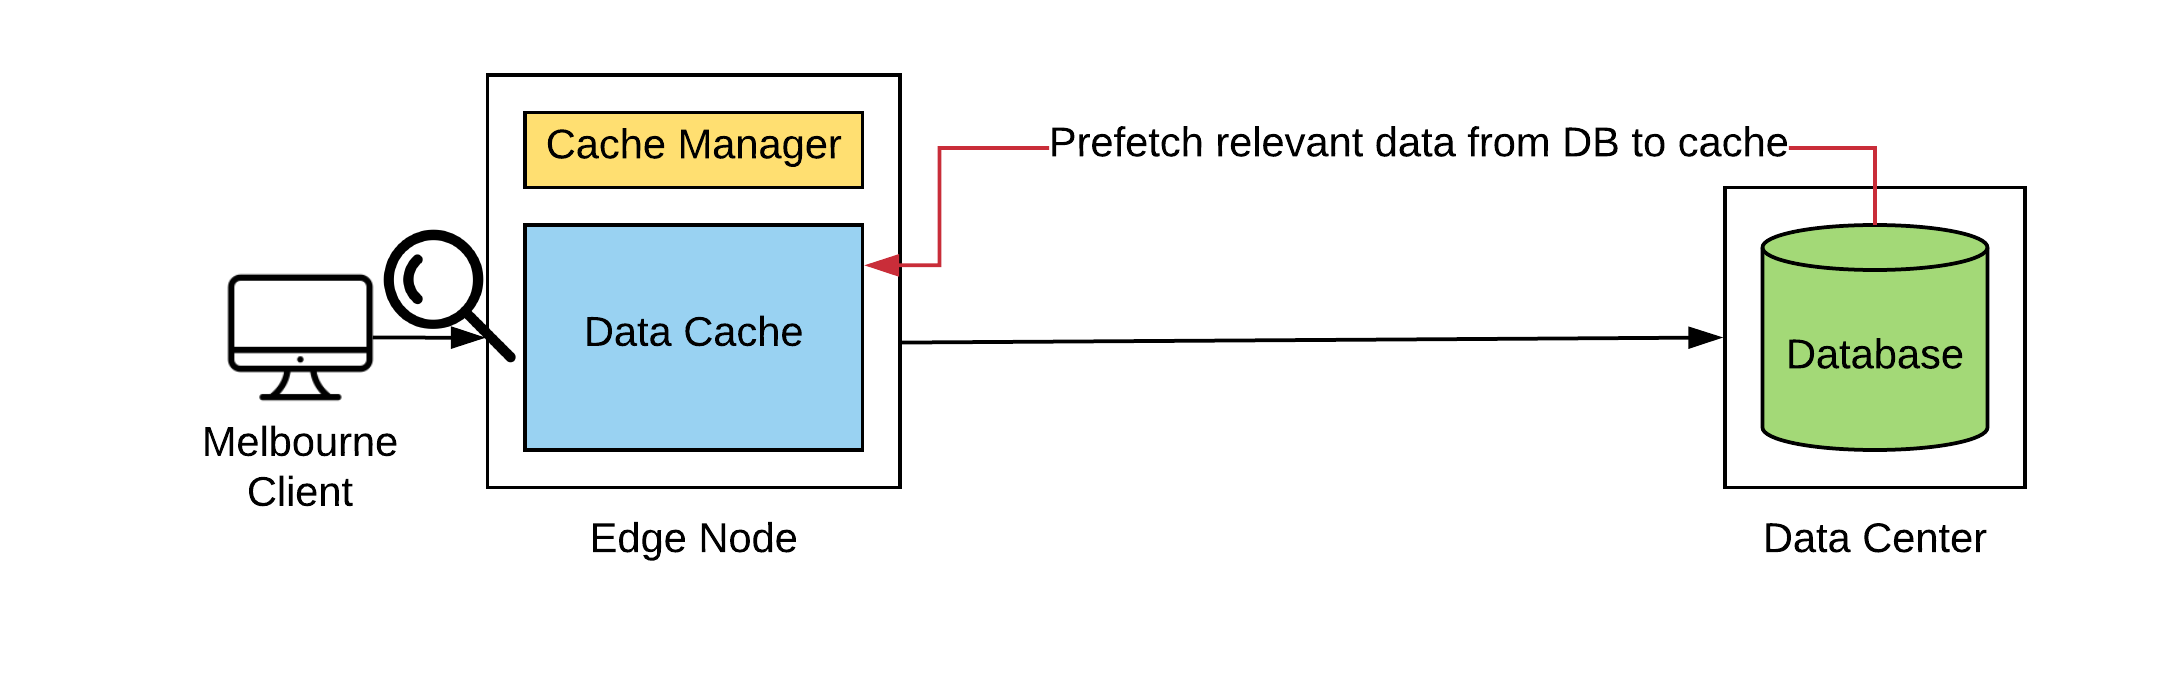
\includegraphics[scale=0.17]{apollo_ec_dbl_learn}
    \end{figure}
\end{frame}

\begin{frame}{Query Patterns}
    Execution of a query informs which queries will execute next, and
    with what parameters.
\end{frame}

\begin{frame}[fragile]{Dynamic Data Requests (TPC-W Benchmark)}
    \begin{lstlisting}[
                   language=SQL,
                   basicstyle=\ttfamily,
                   commentstyle=\color{gray},
                   escapeinside={(*@}{@*)},
                ]
1. SELECT (*@ \cfbox{red}{C\_ID} @*) FROM CUSTOMER WHERE 
C_UNAME = @C_UN and C_PASSWD = @C_PAS

2. SELECT MAX(O_ID) FROM ORDERS WHERE
O_C_ID = (*@ \cfbox{red}{@C\_ID} @*)
    \end{lstlisting}

\begin{center}
\end{center}
\end{frame}

\begin{frame}{Predictive Caching}
    \begin{figure}
        \center
        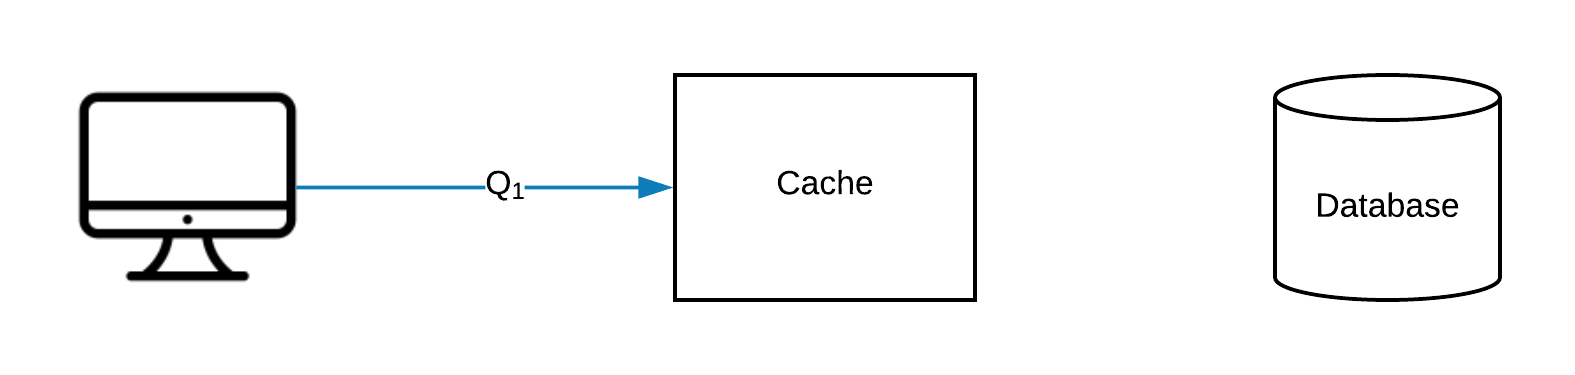
\includegraphics[scale=0.17]{apollo_predictive_execution}
    \end{figure}
\end{frame}

\begin{frame}{Predictive Caching}
    \begin{figure}
        \center
        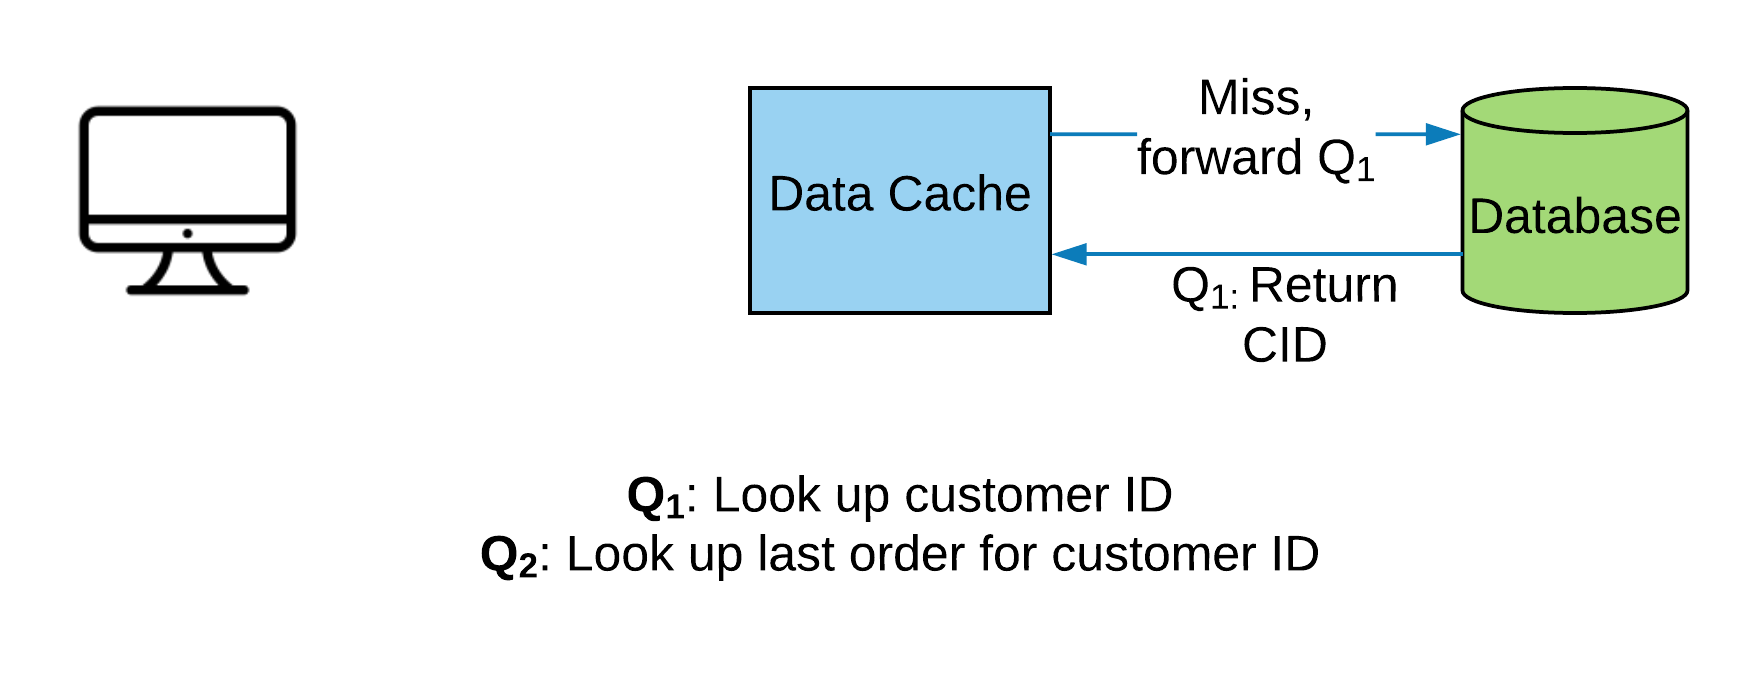
\includegraphics[scale=0.17]{apollo_predictive_execution_2}
    \end{figure}
\end{frame}

\begin{frame}{Predictive Caching}
    \begin{figure}
        \center
        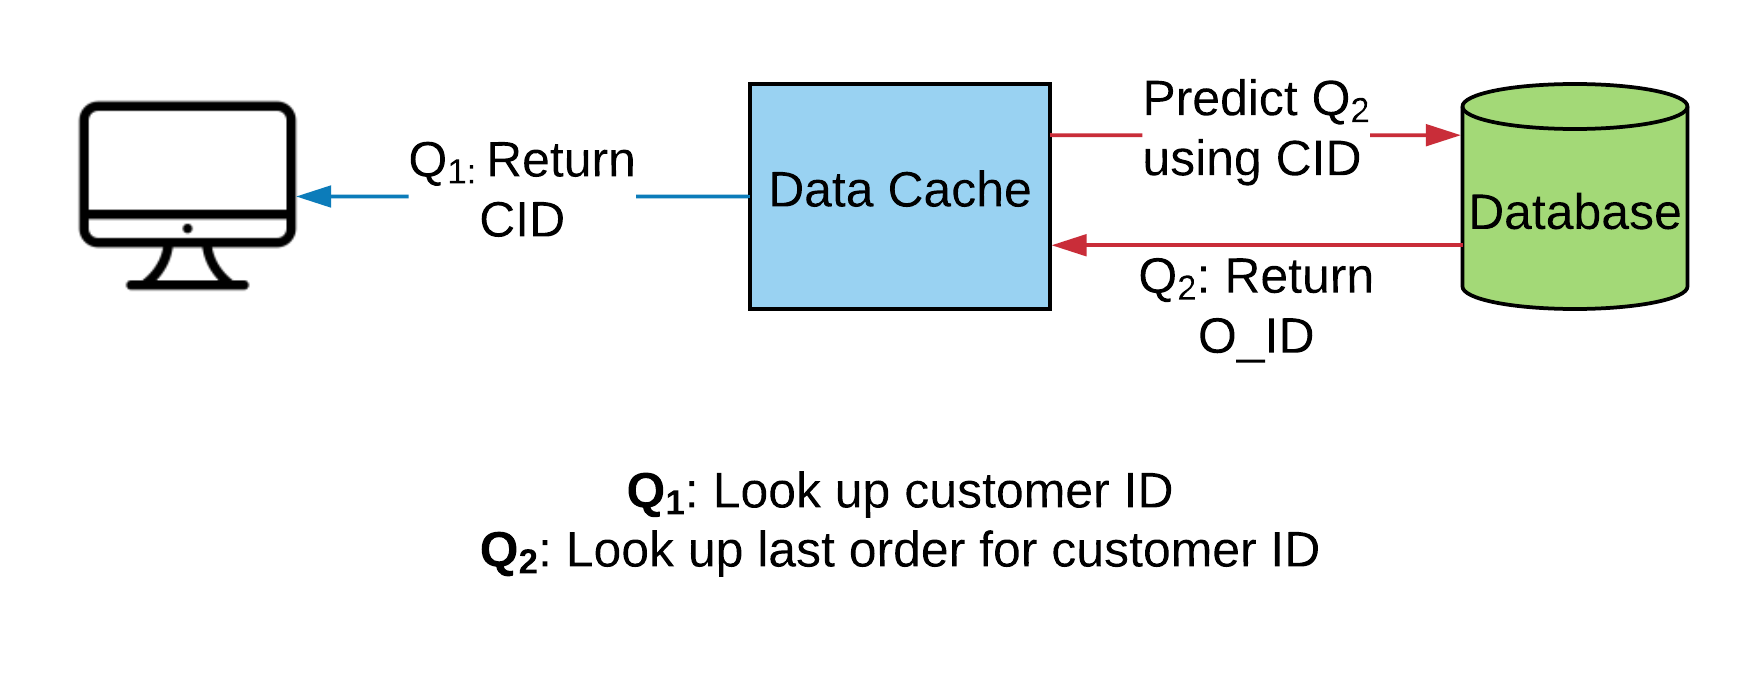
\includegraphics[scale=0.17]{apollo_predictive_execution_4}
    \end{figure}
\end{frame}

\begin{frame}{Predictive Caching}
    \begin{figure}
        \center
        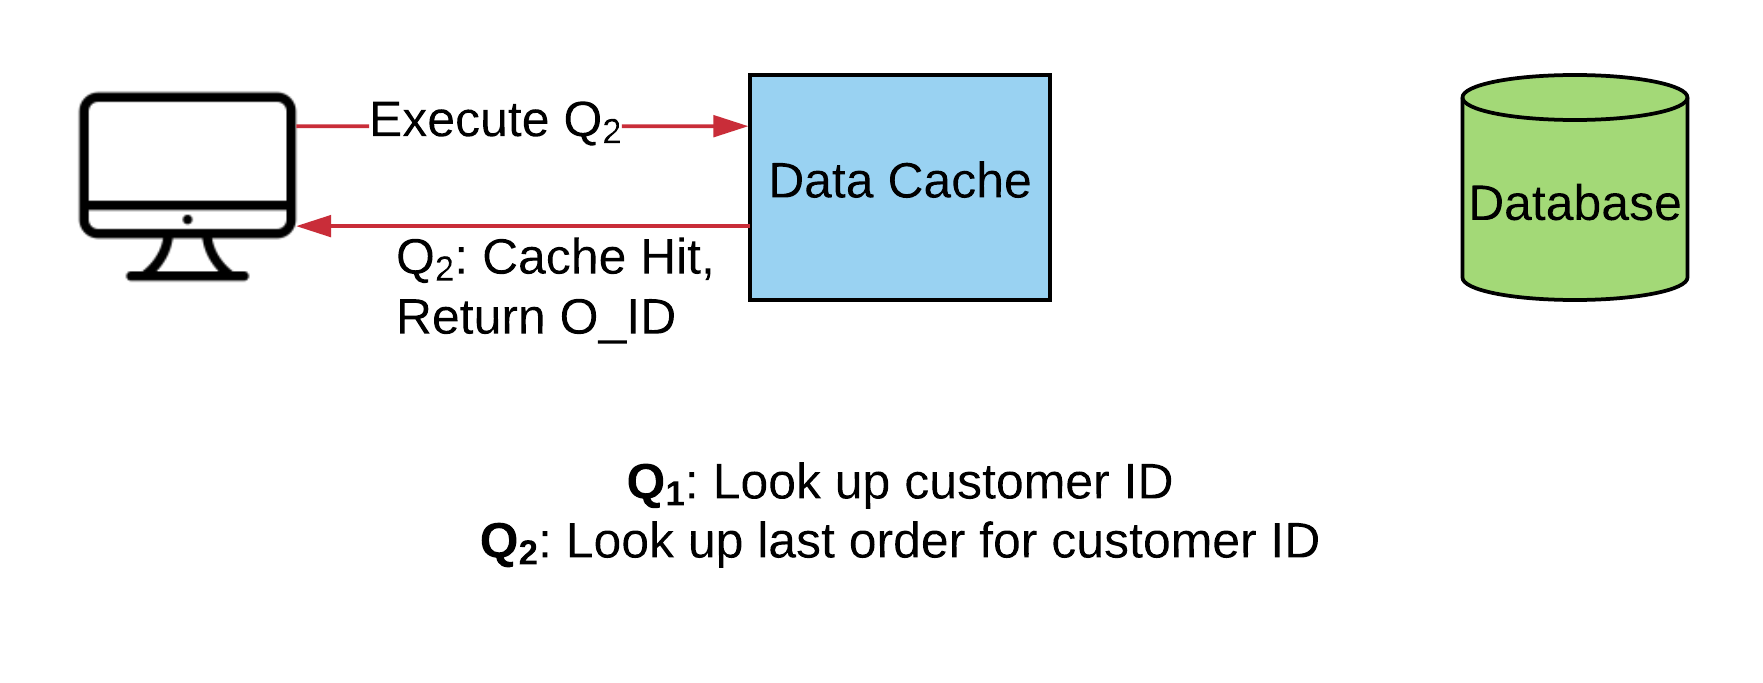
\includegraphics[scale=0.17]{apollo_predictive_execution_5}
    \end{figure}
\end{frame}

\begin{frame}{Apollo: Caching Dynamic Data on a Global Scale}
    We developed Apollo, a middleware system that:
    \begin{itemize}
        \visible<2->{
            \item{Uses \alert{online learning} to adapt cache behaviour based on client behaviour patterns.}
        }
        \visible<3->{
            \item{\alert{Predictively executes} and caches query results to reduce client response time.}
        }
        \visible<4->{
            \item{Employs a \alert{computationally efficient} means of managing updates to cached data at global scale.}
        }
    \end{itemize}
\end{frame}

\begin{frame}{Table of contents}
  \setbeamertemplate{section in toc}[sections numbered]
  \tableofcontents[hideallsubsections]
\end{frame}

\section{Predictive Query Model}

\begin{frame}[fragile]{Apollo Overview}
    \begin{figure}
        \hspace*{-1cm}
        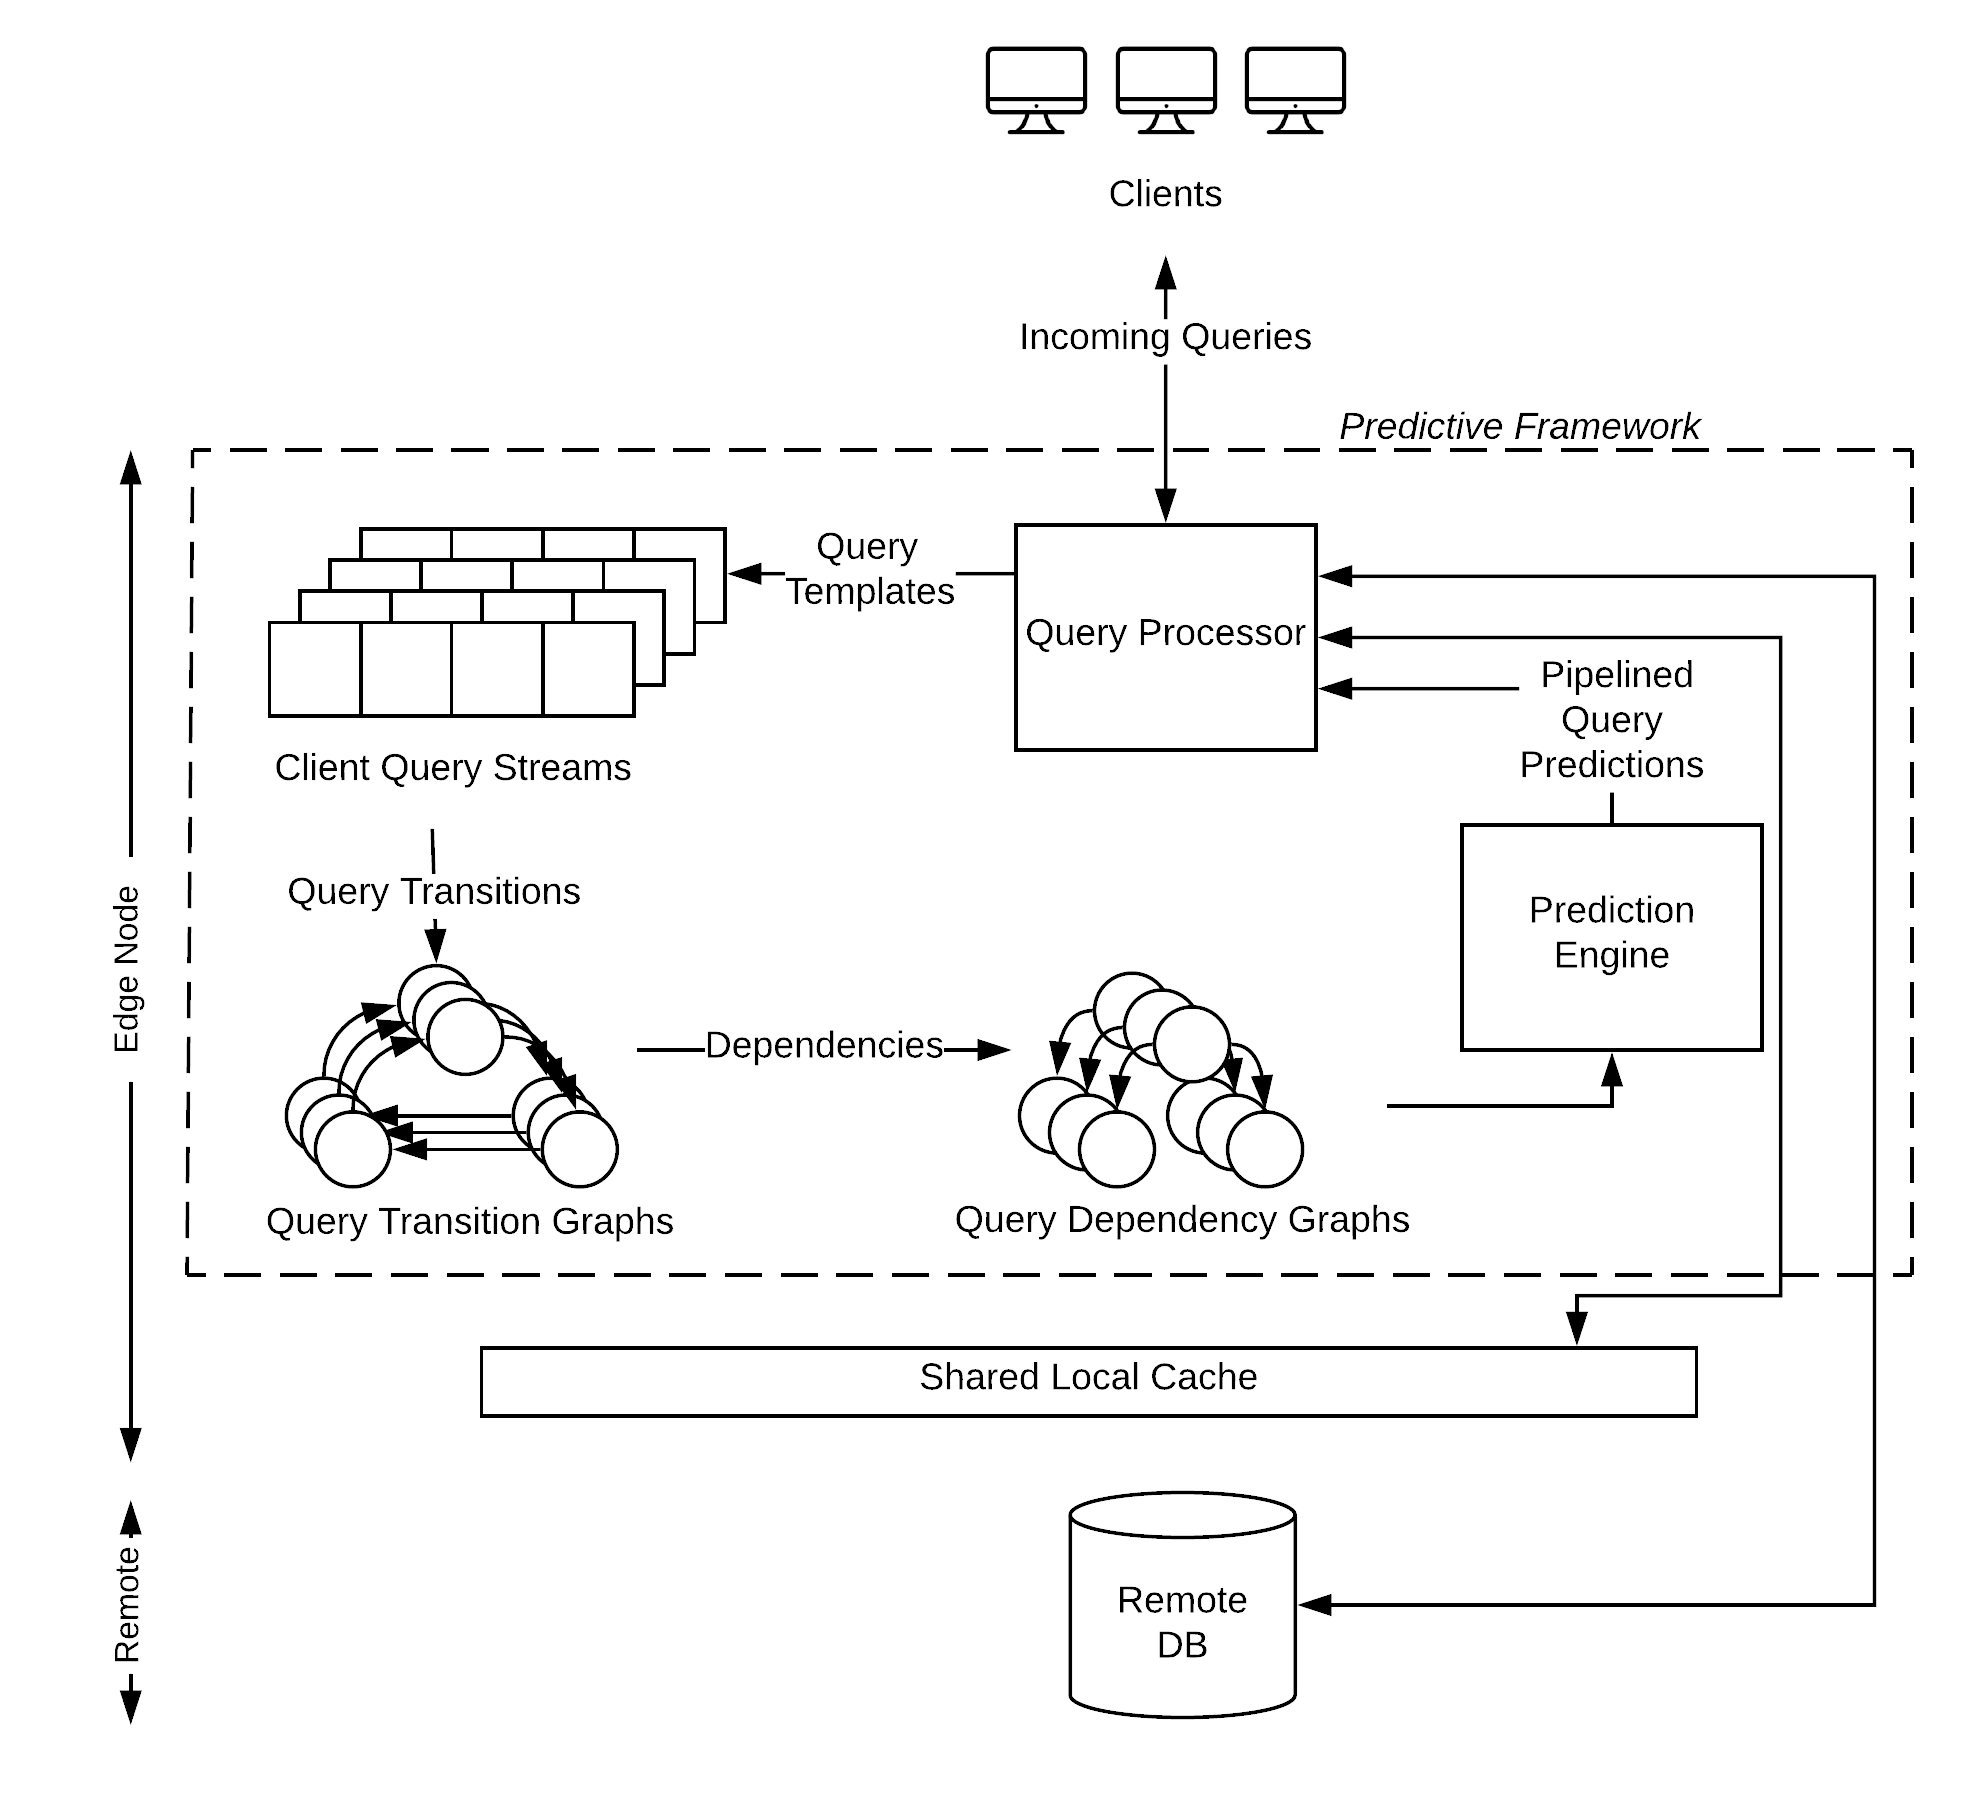
\includegraphics[scale=0.13]{apollo_overview}
    \end{figure}
\end{frame}

\begin{frame}[fragile]{Apollo Overview}
    \begin{figure}
        \hspace*{-1cm}
        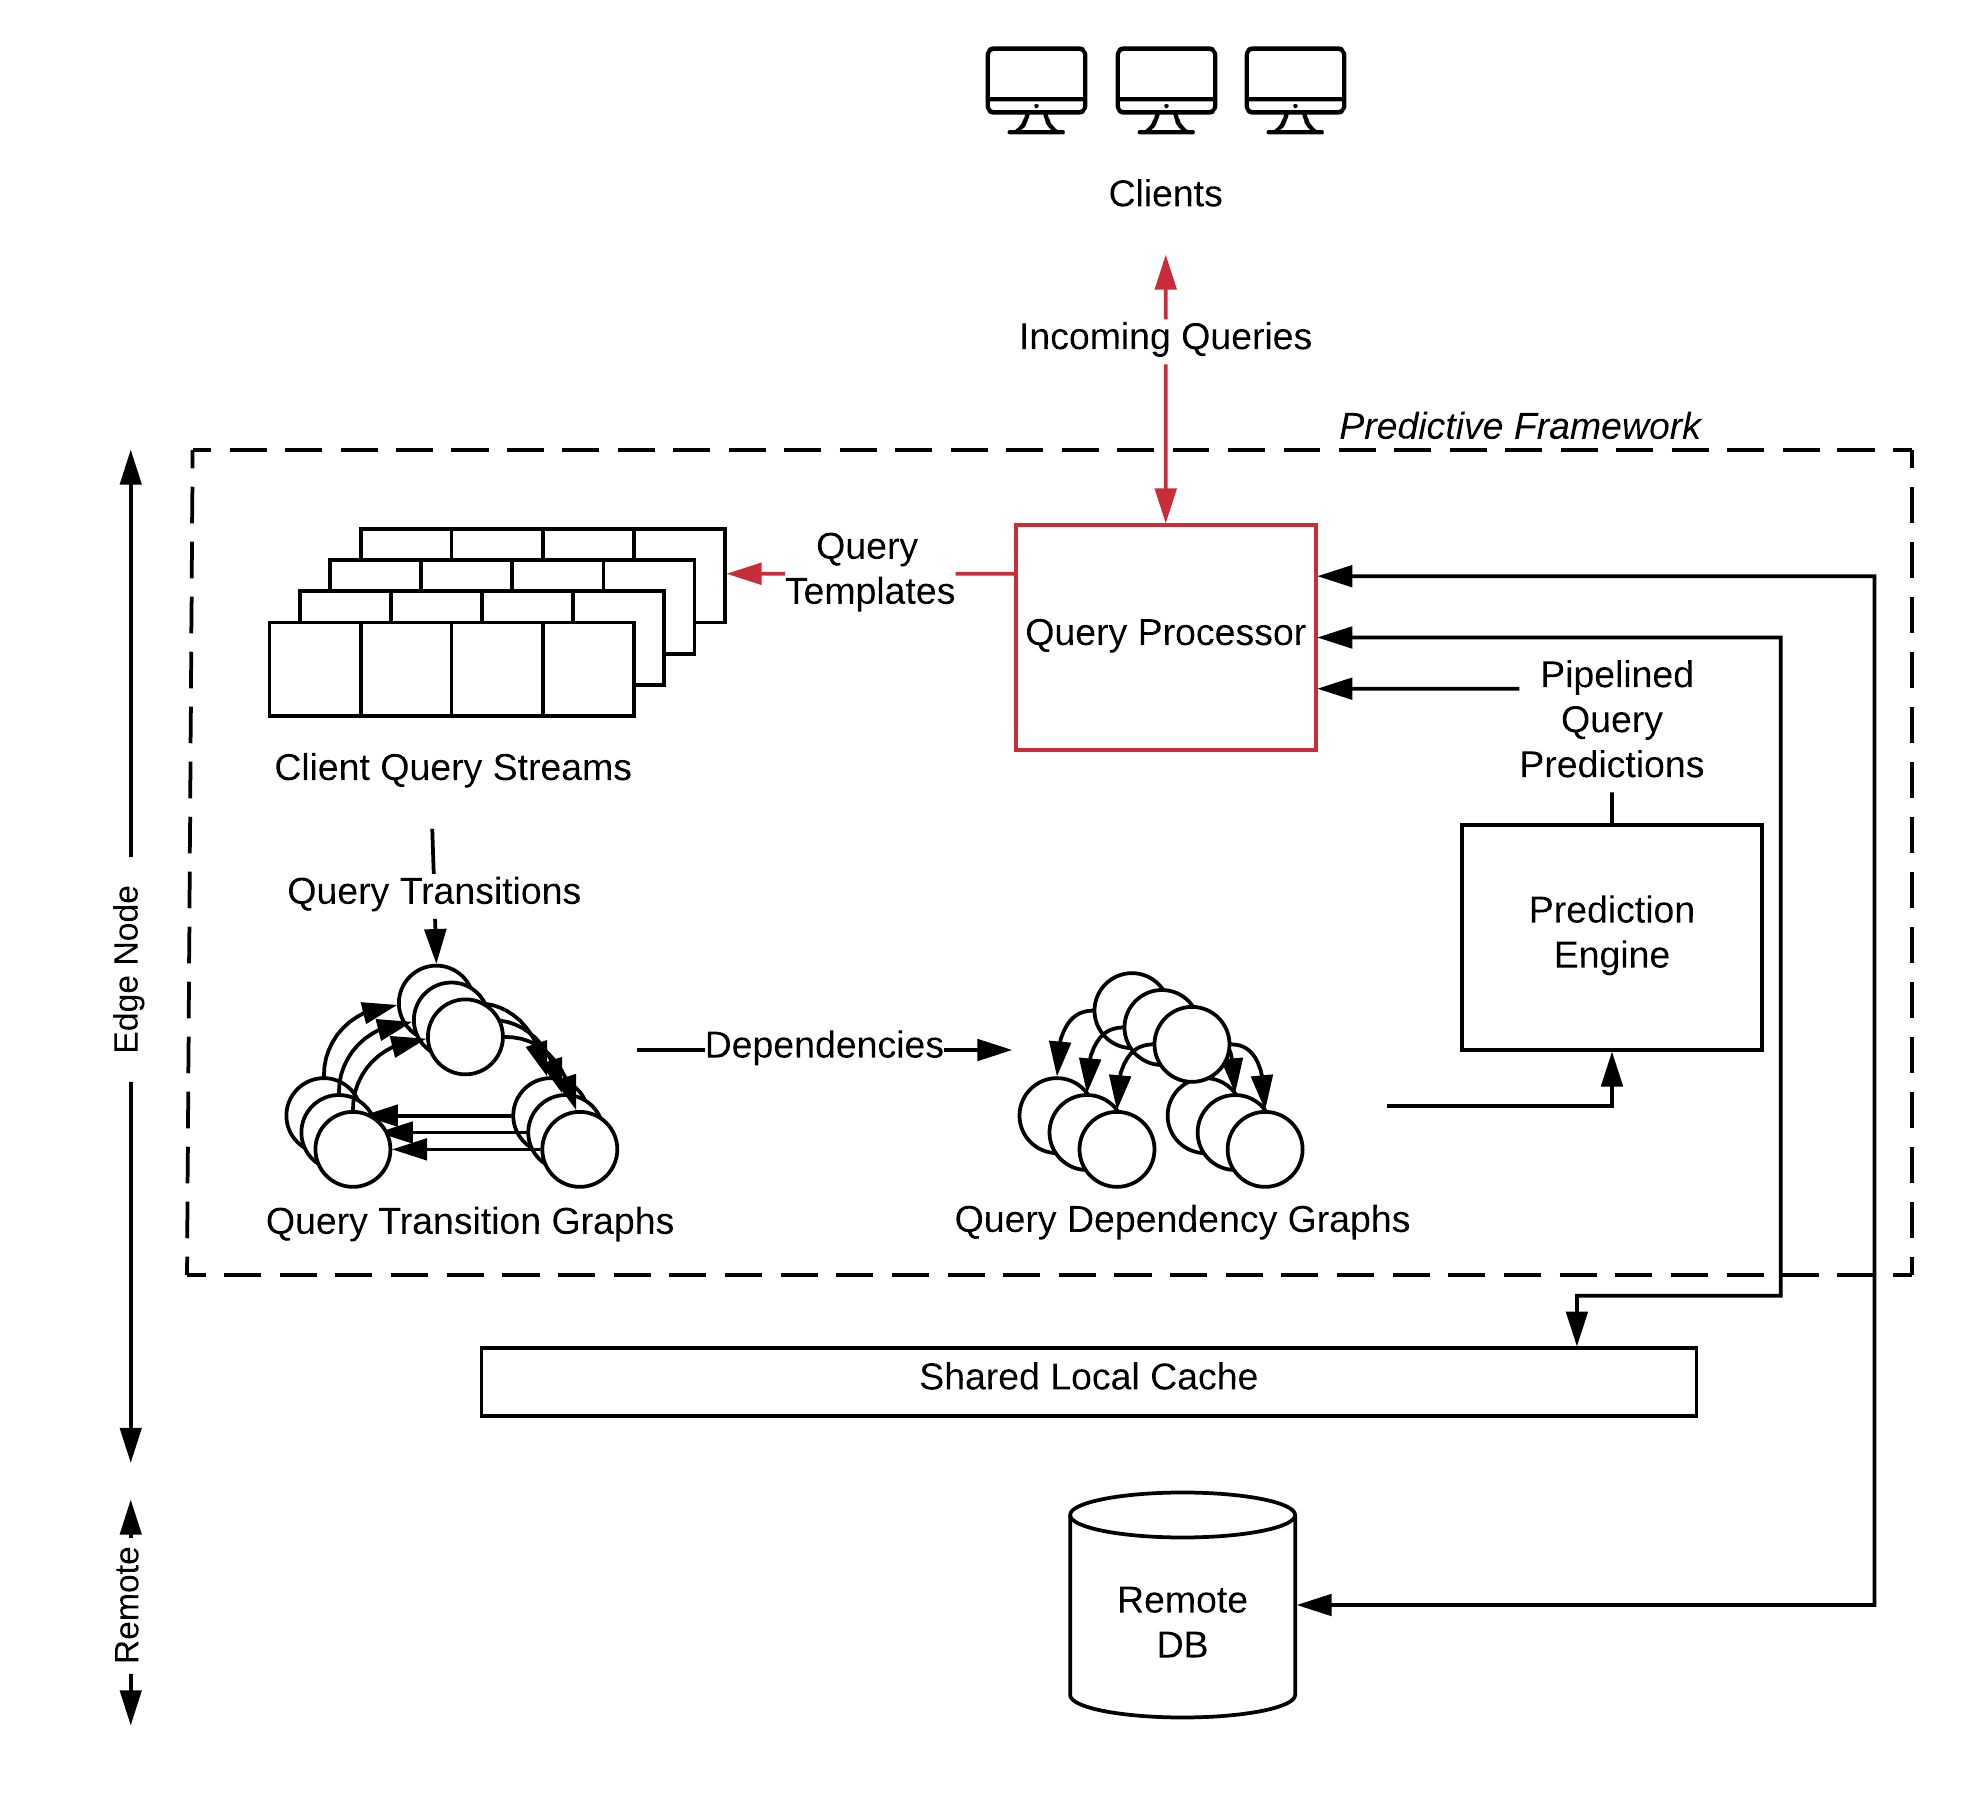
\includegraphics[scale=0.13]{apollo_overview_2}
    \end{figure}
\end{frame}

\begin{frame}[fragile]{Apollo Overview}
    \begin{figure}
        \hspace*{-1cm}
        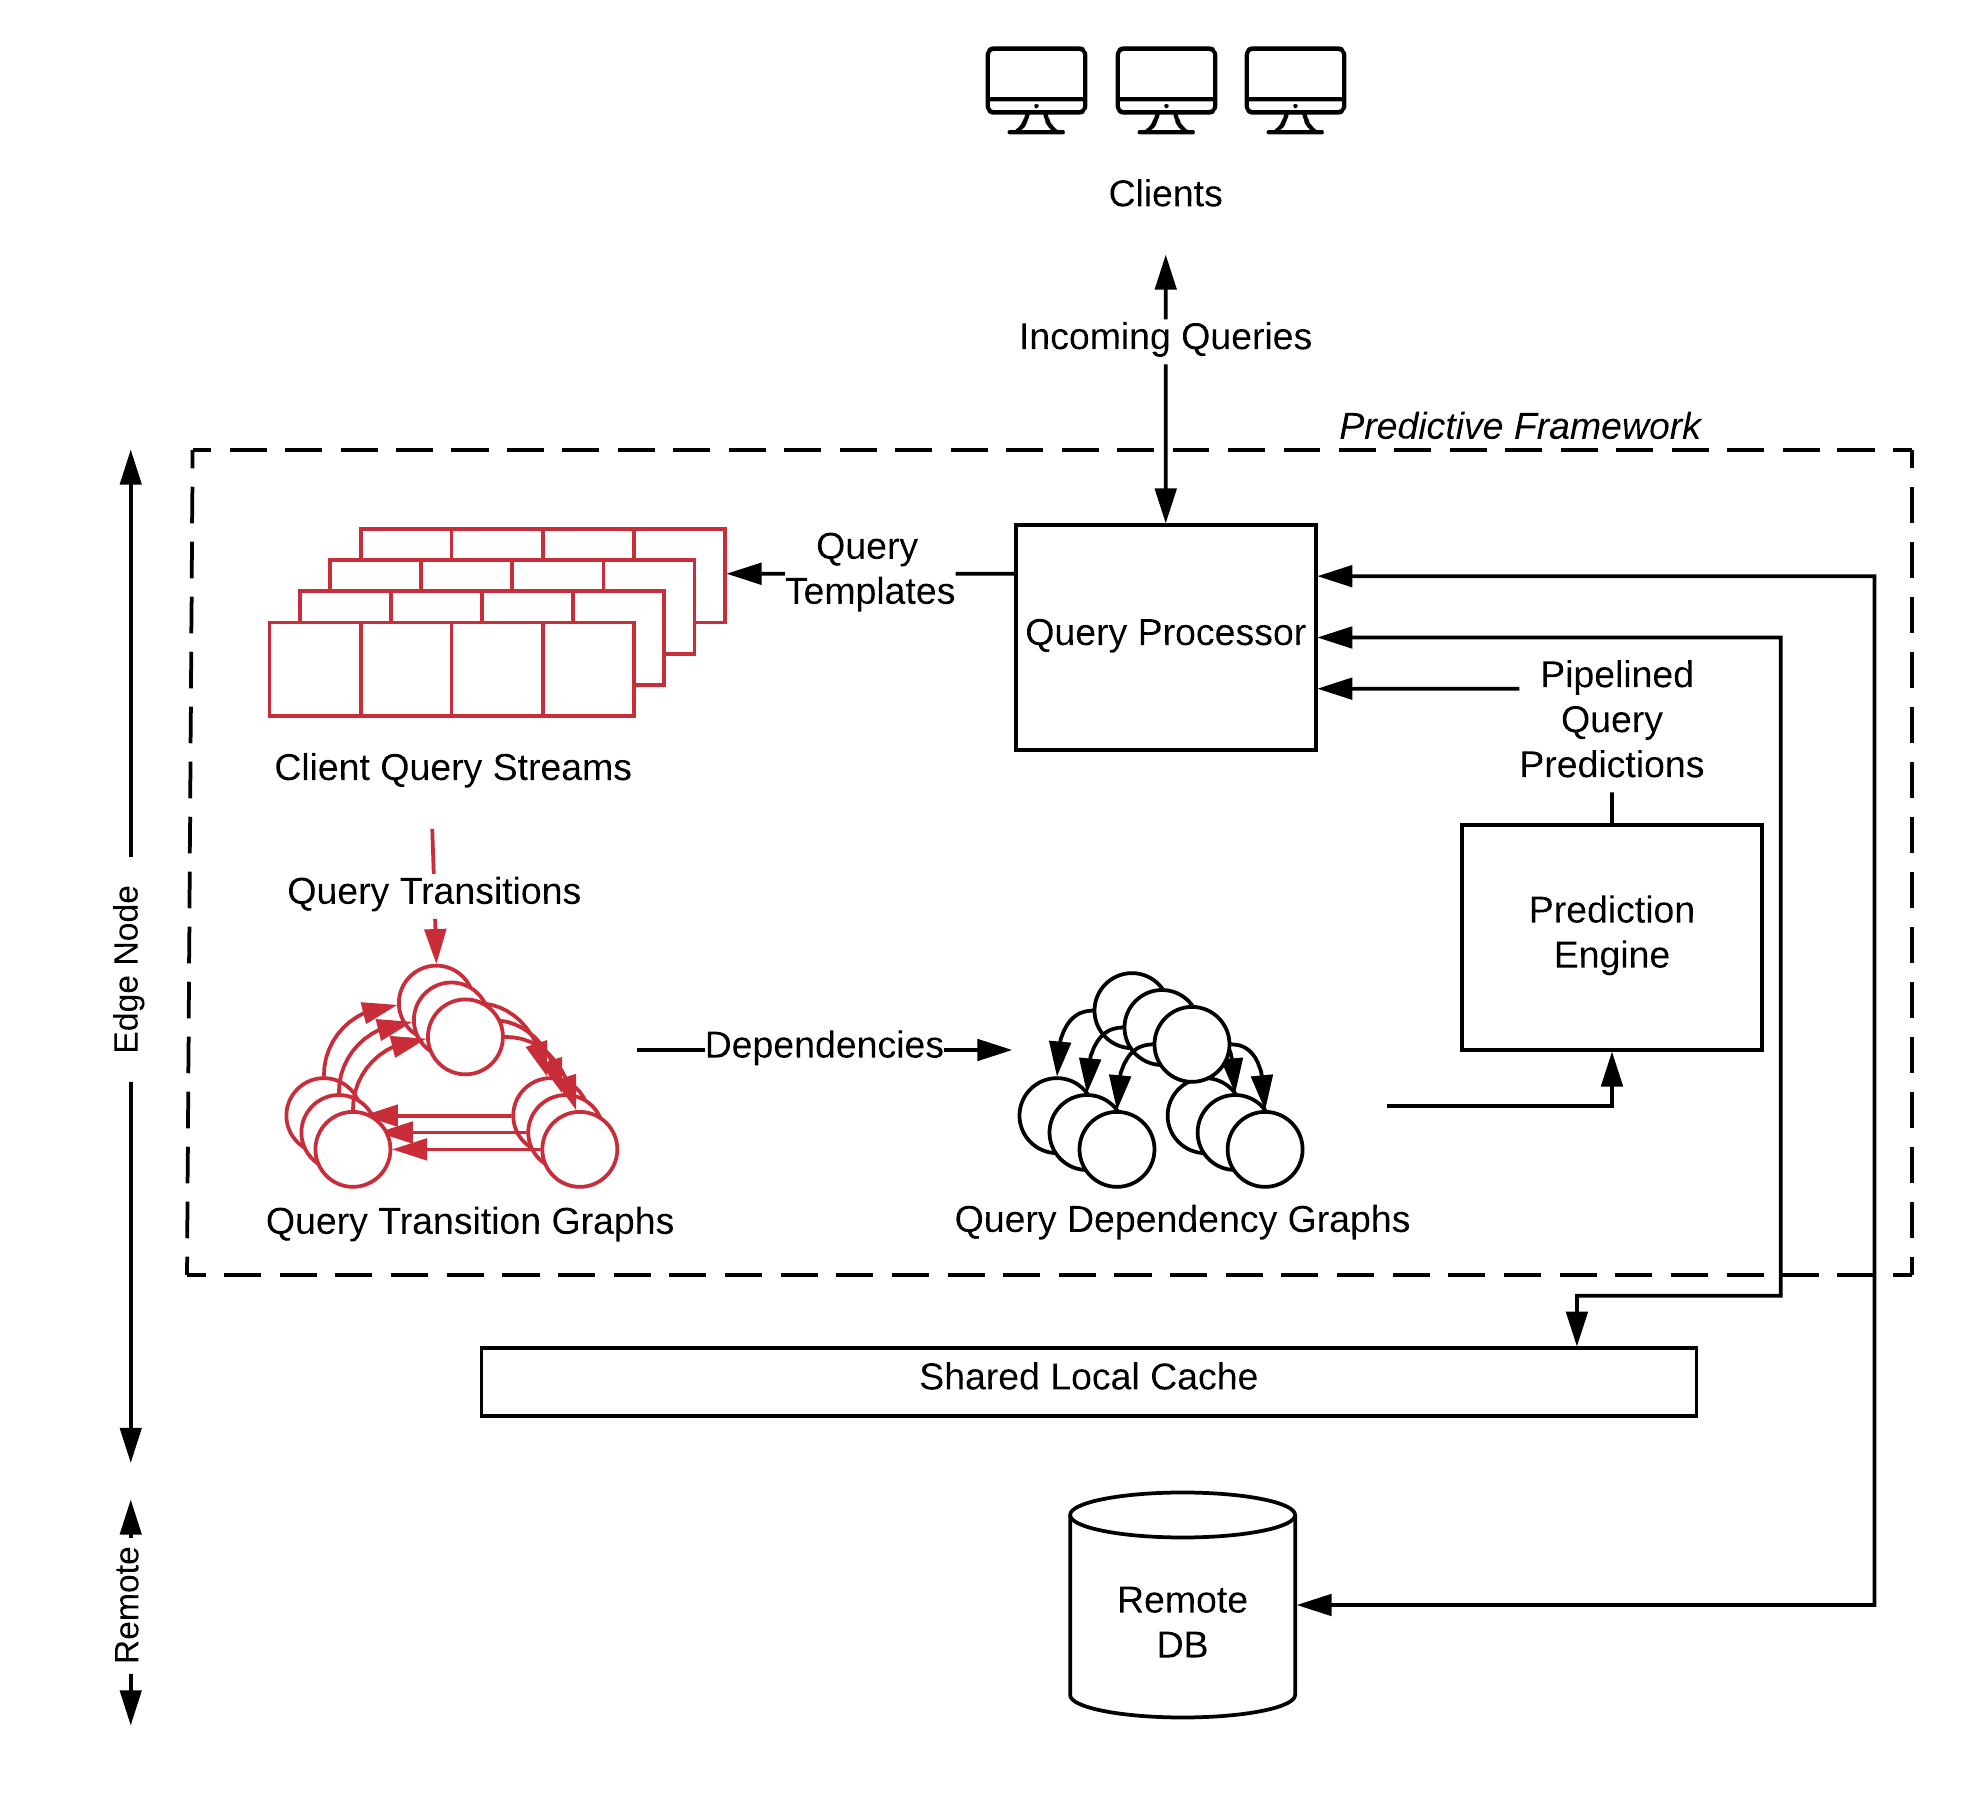
\includegraphics[scale=0.13]{apollo_overview_3}
    \end{figure}
\end{frame}

\begin{frame}[fragile]{Apollo Overview}
    \begin{figure}
        \hspace*{-1cm}
        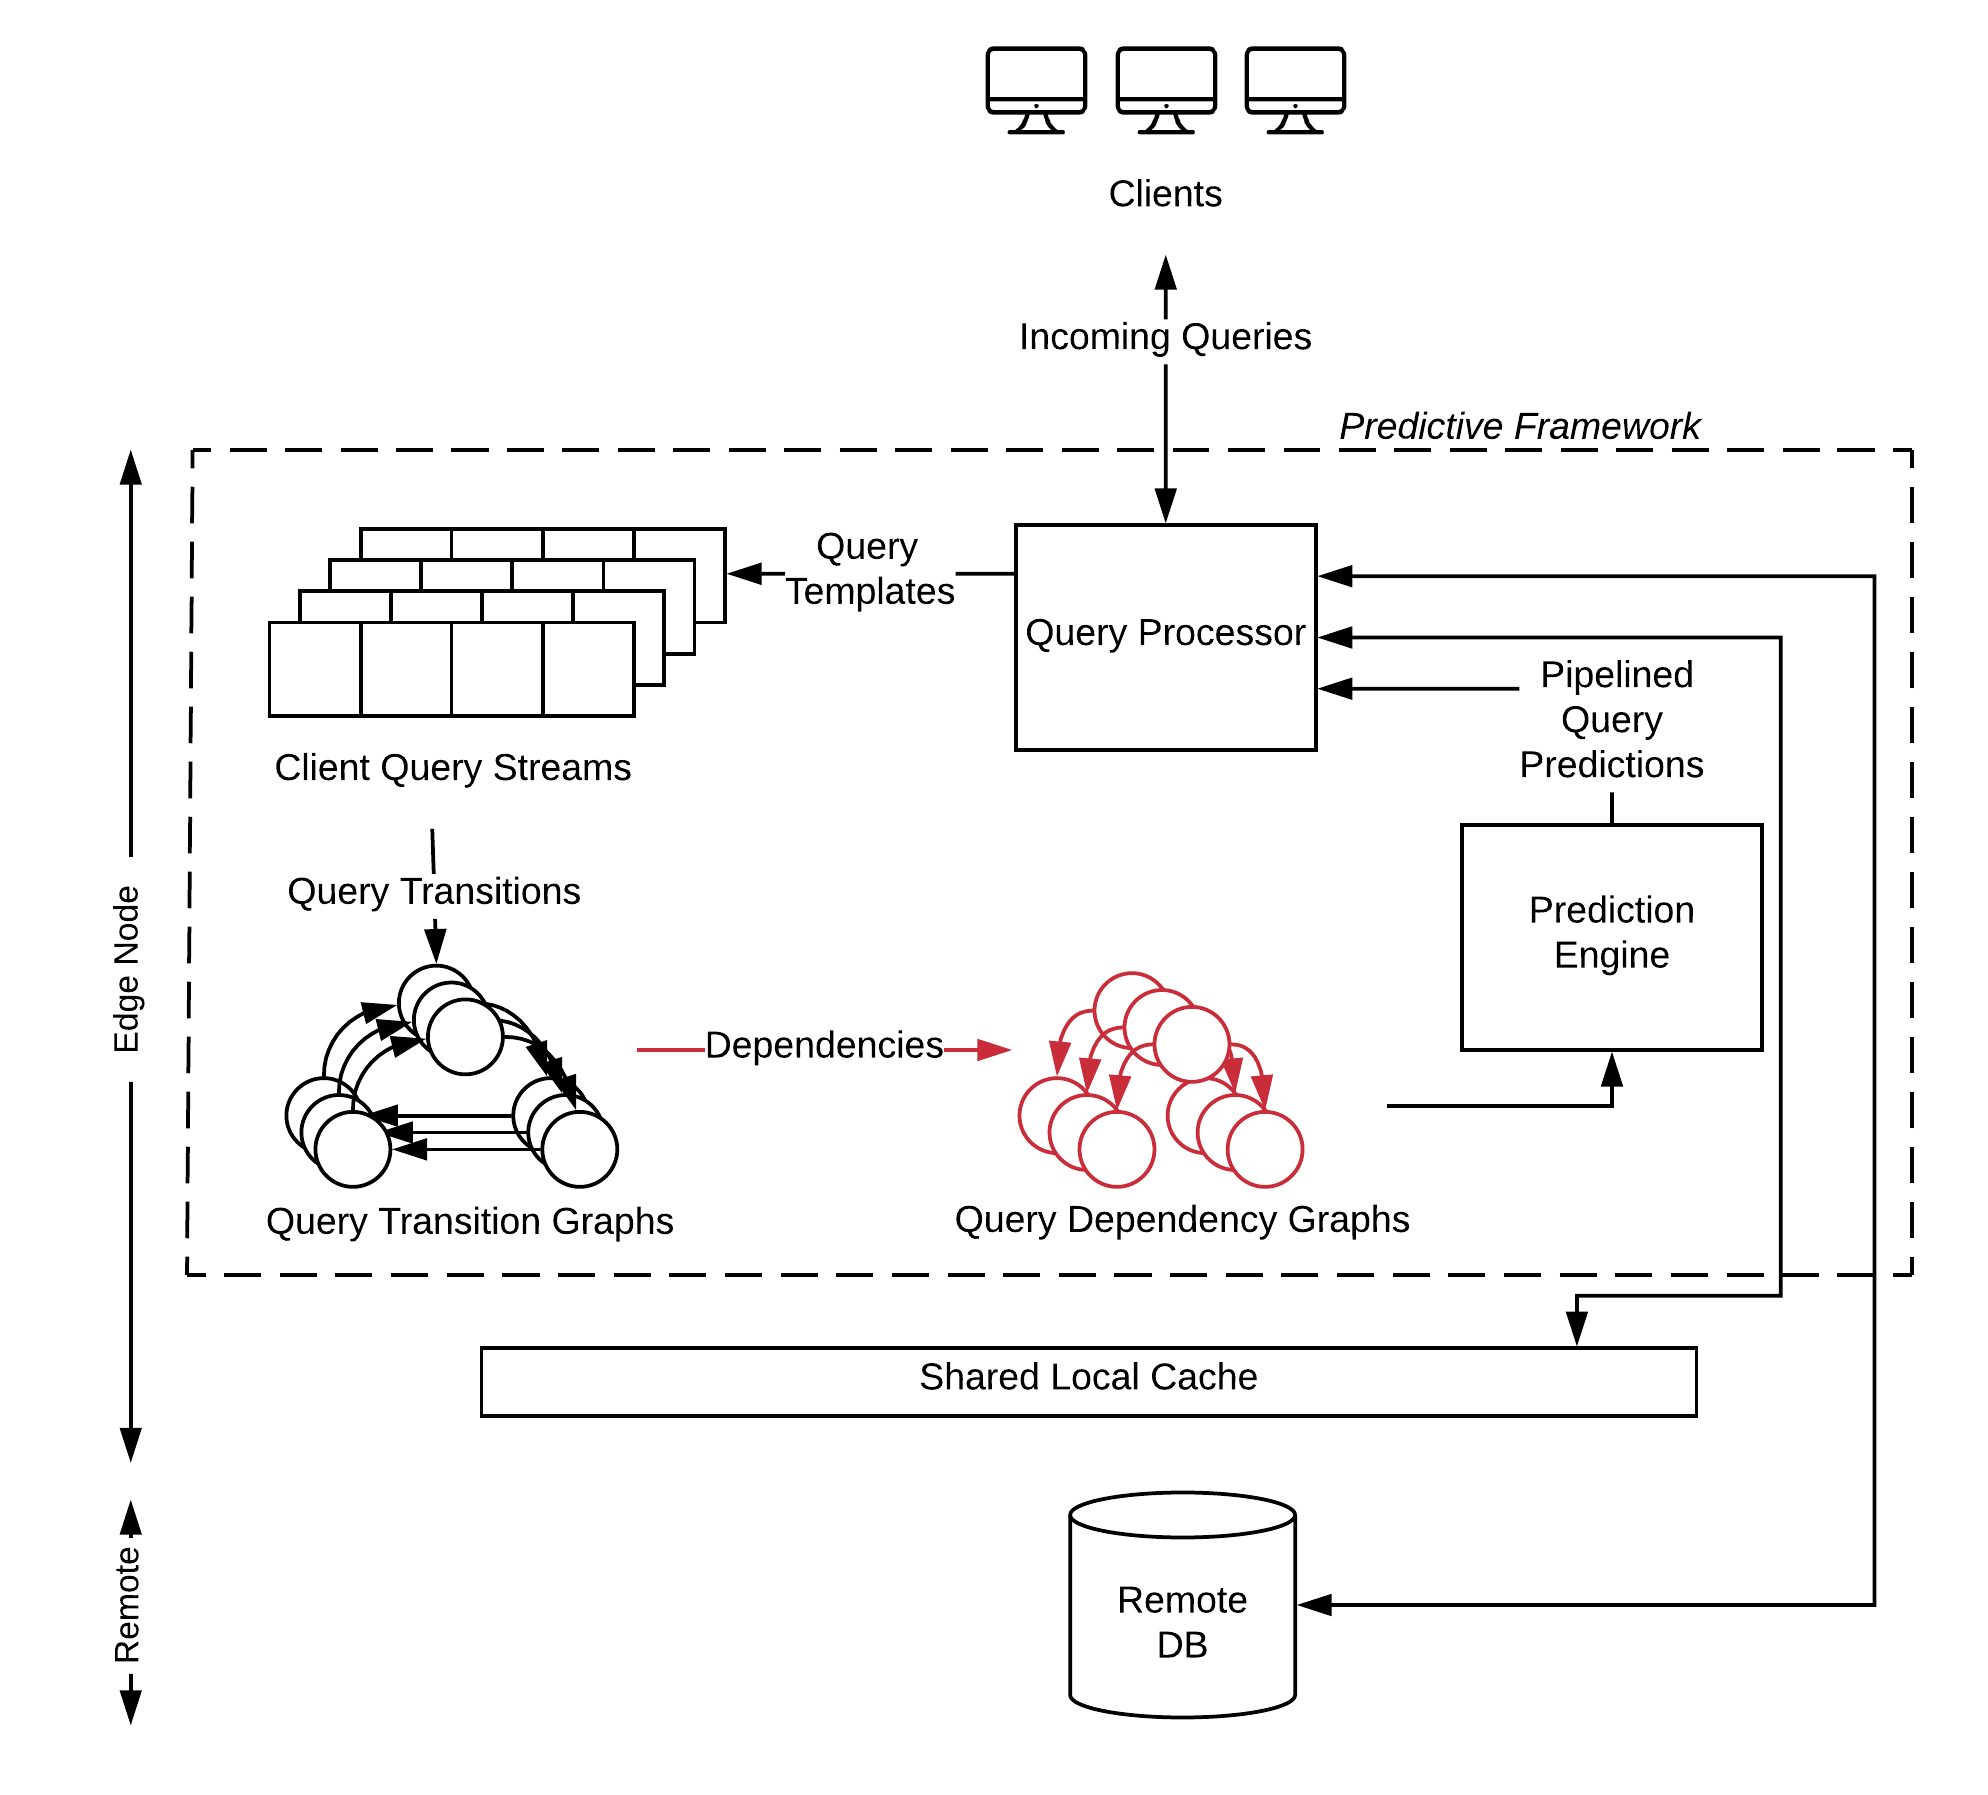
\includegraphics[scale=0.13]{apollo_overview_4}
    \end{figure}
\end{frame}

\begin{frame}[fragile]{Apollo Overview}
    \begin{figure}
        \hspace*{-1cm}
        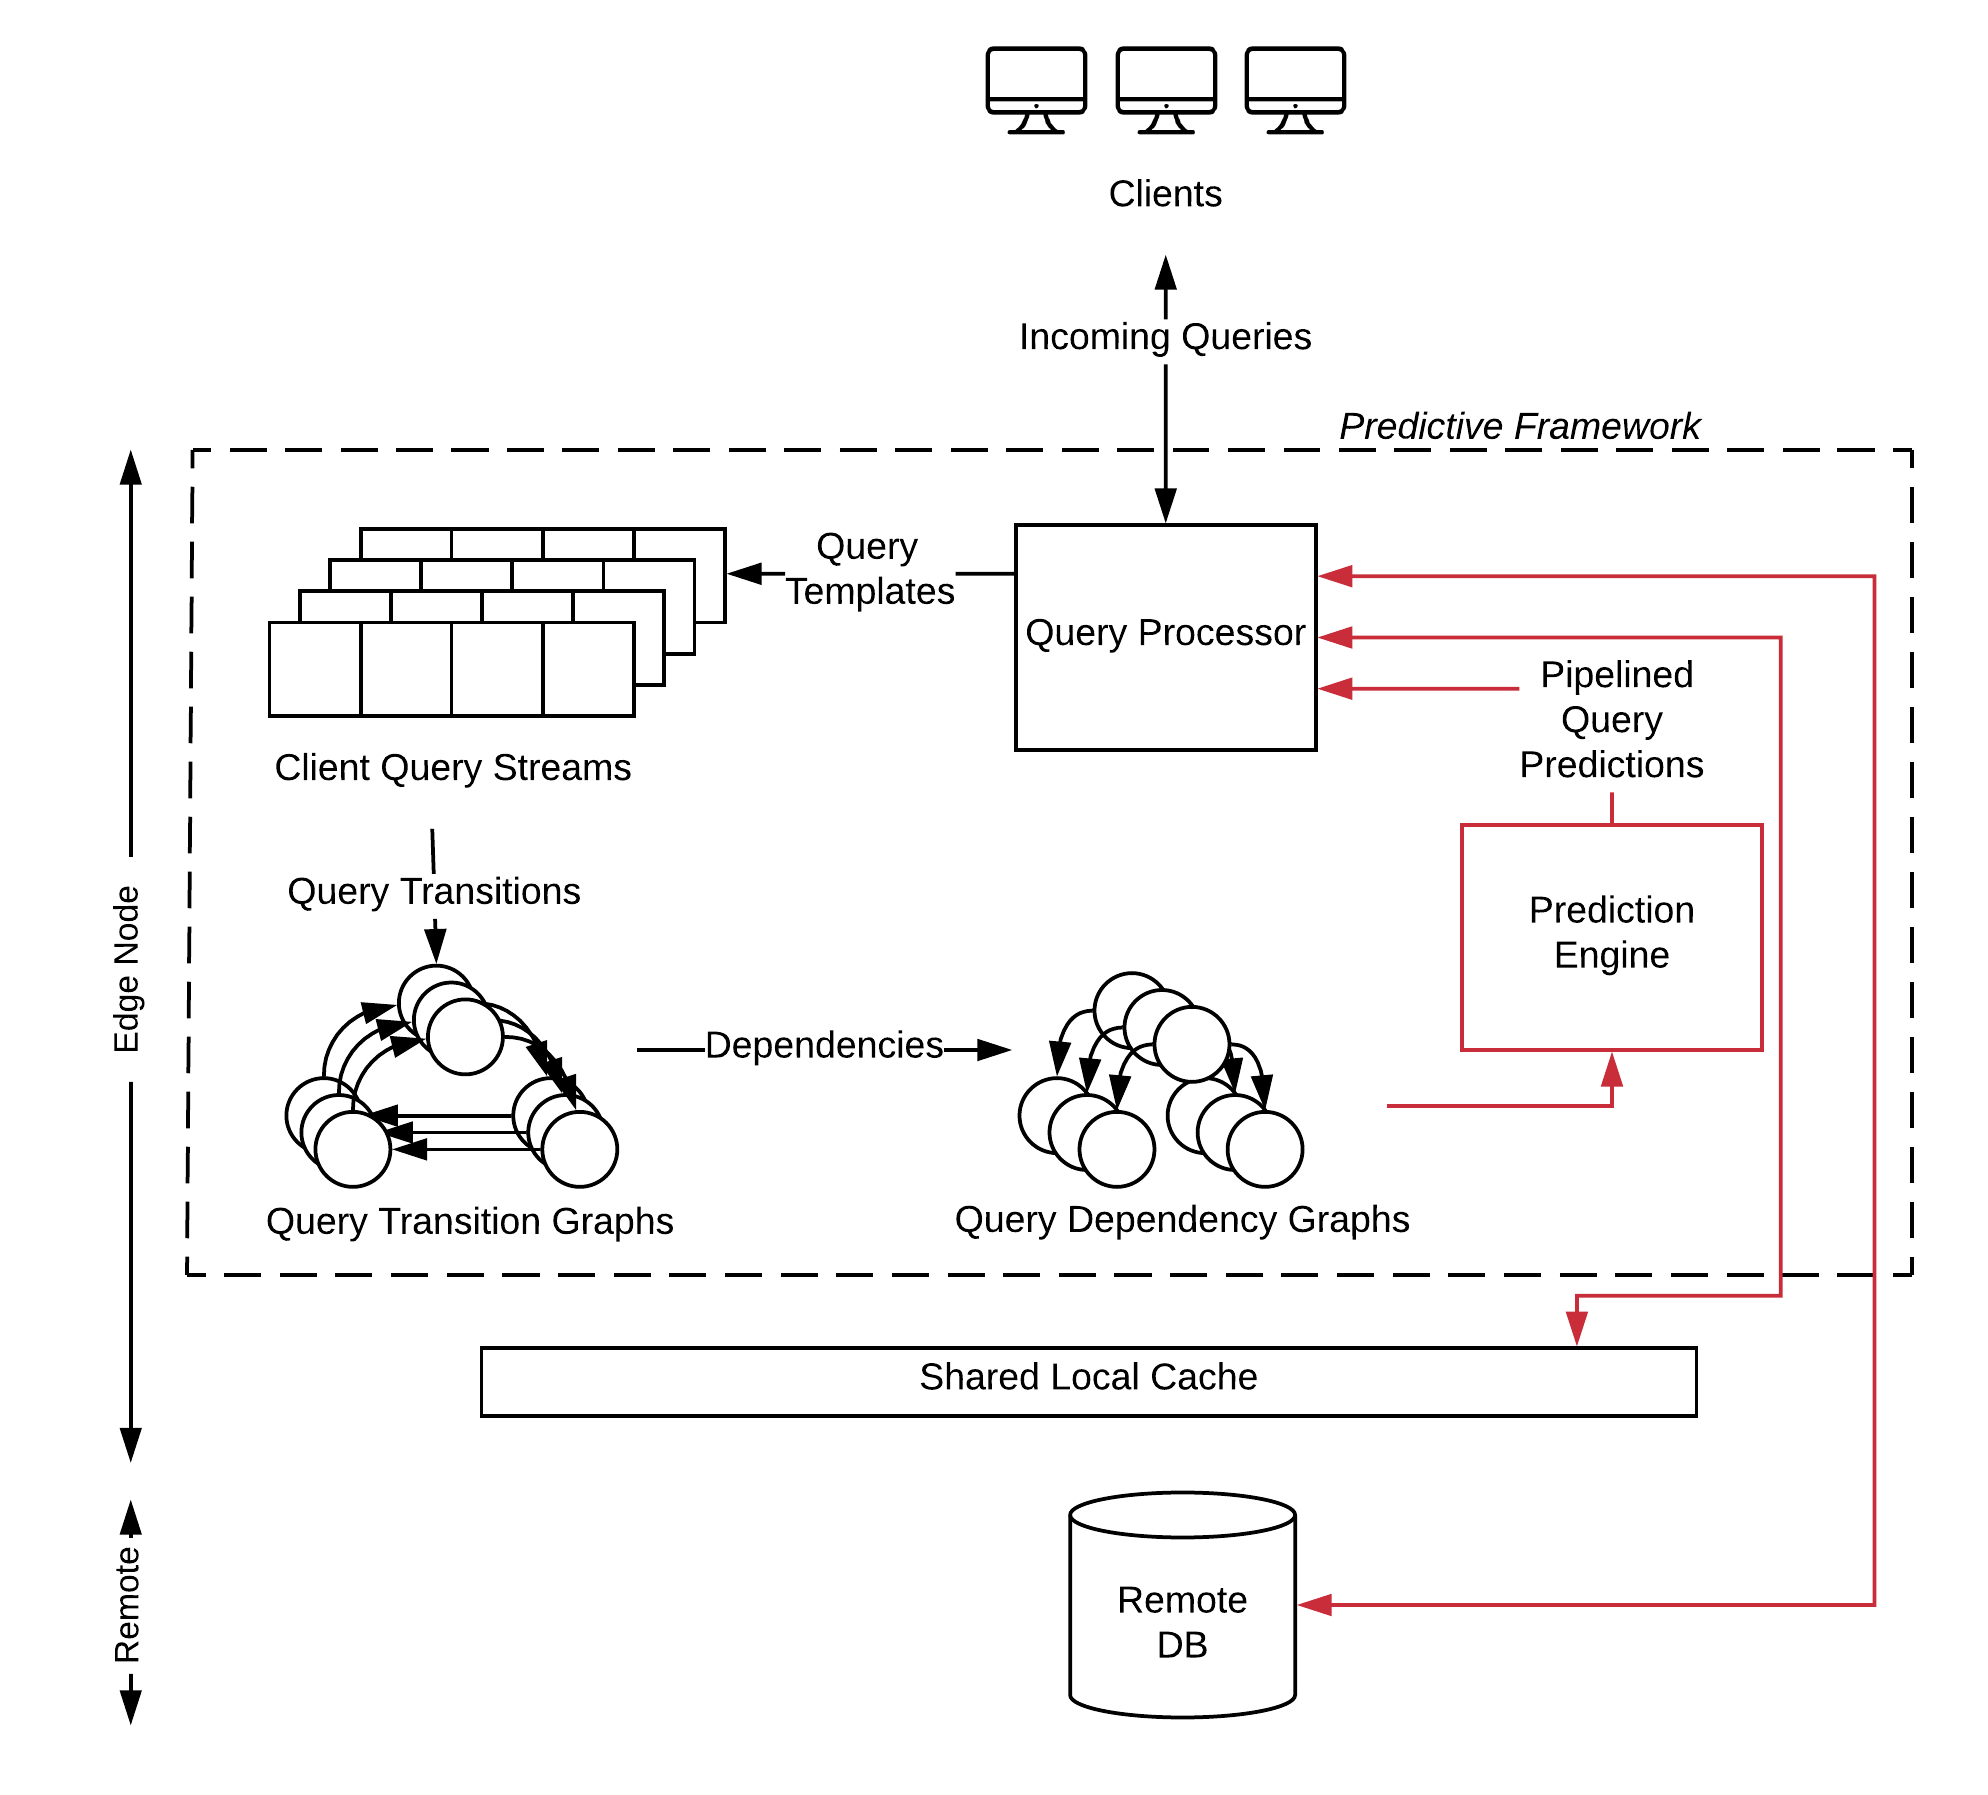
\includegraphics[scale=0.13]{apollo_overview_5}
    \end{figure}
\end{frame}

\begin{frame}[fragile]{Apollo Overview}
    \begin{figure}
        \hspace*{-1cm}
        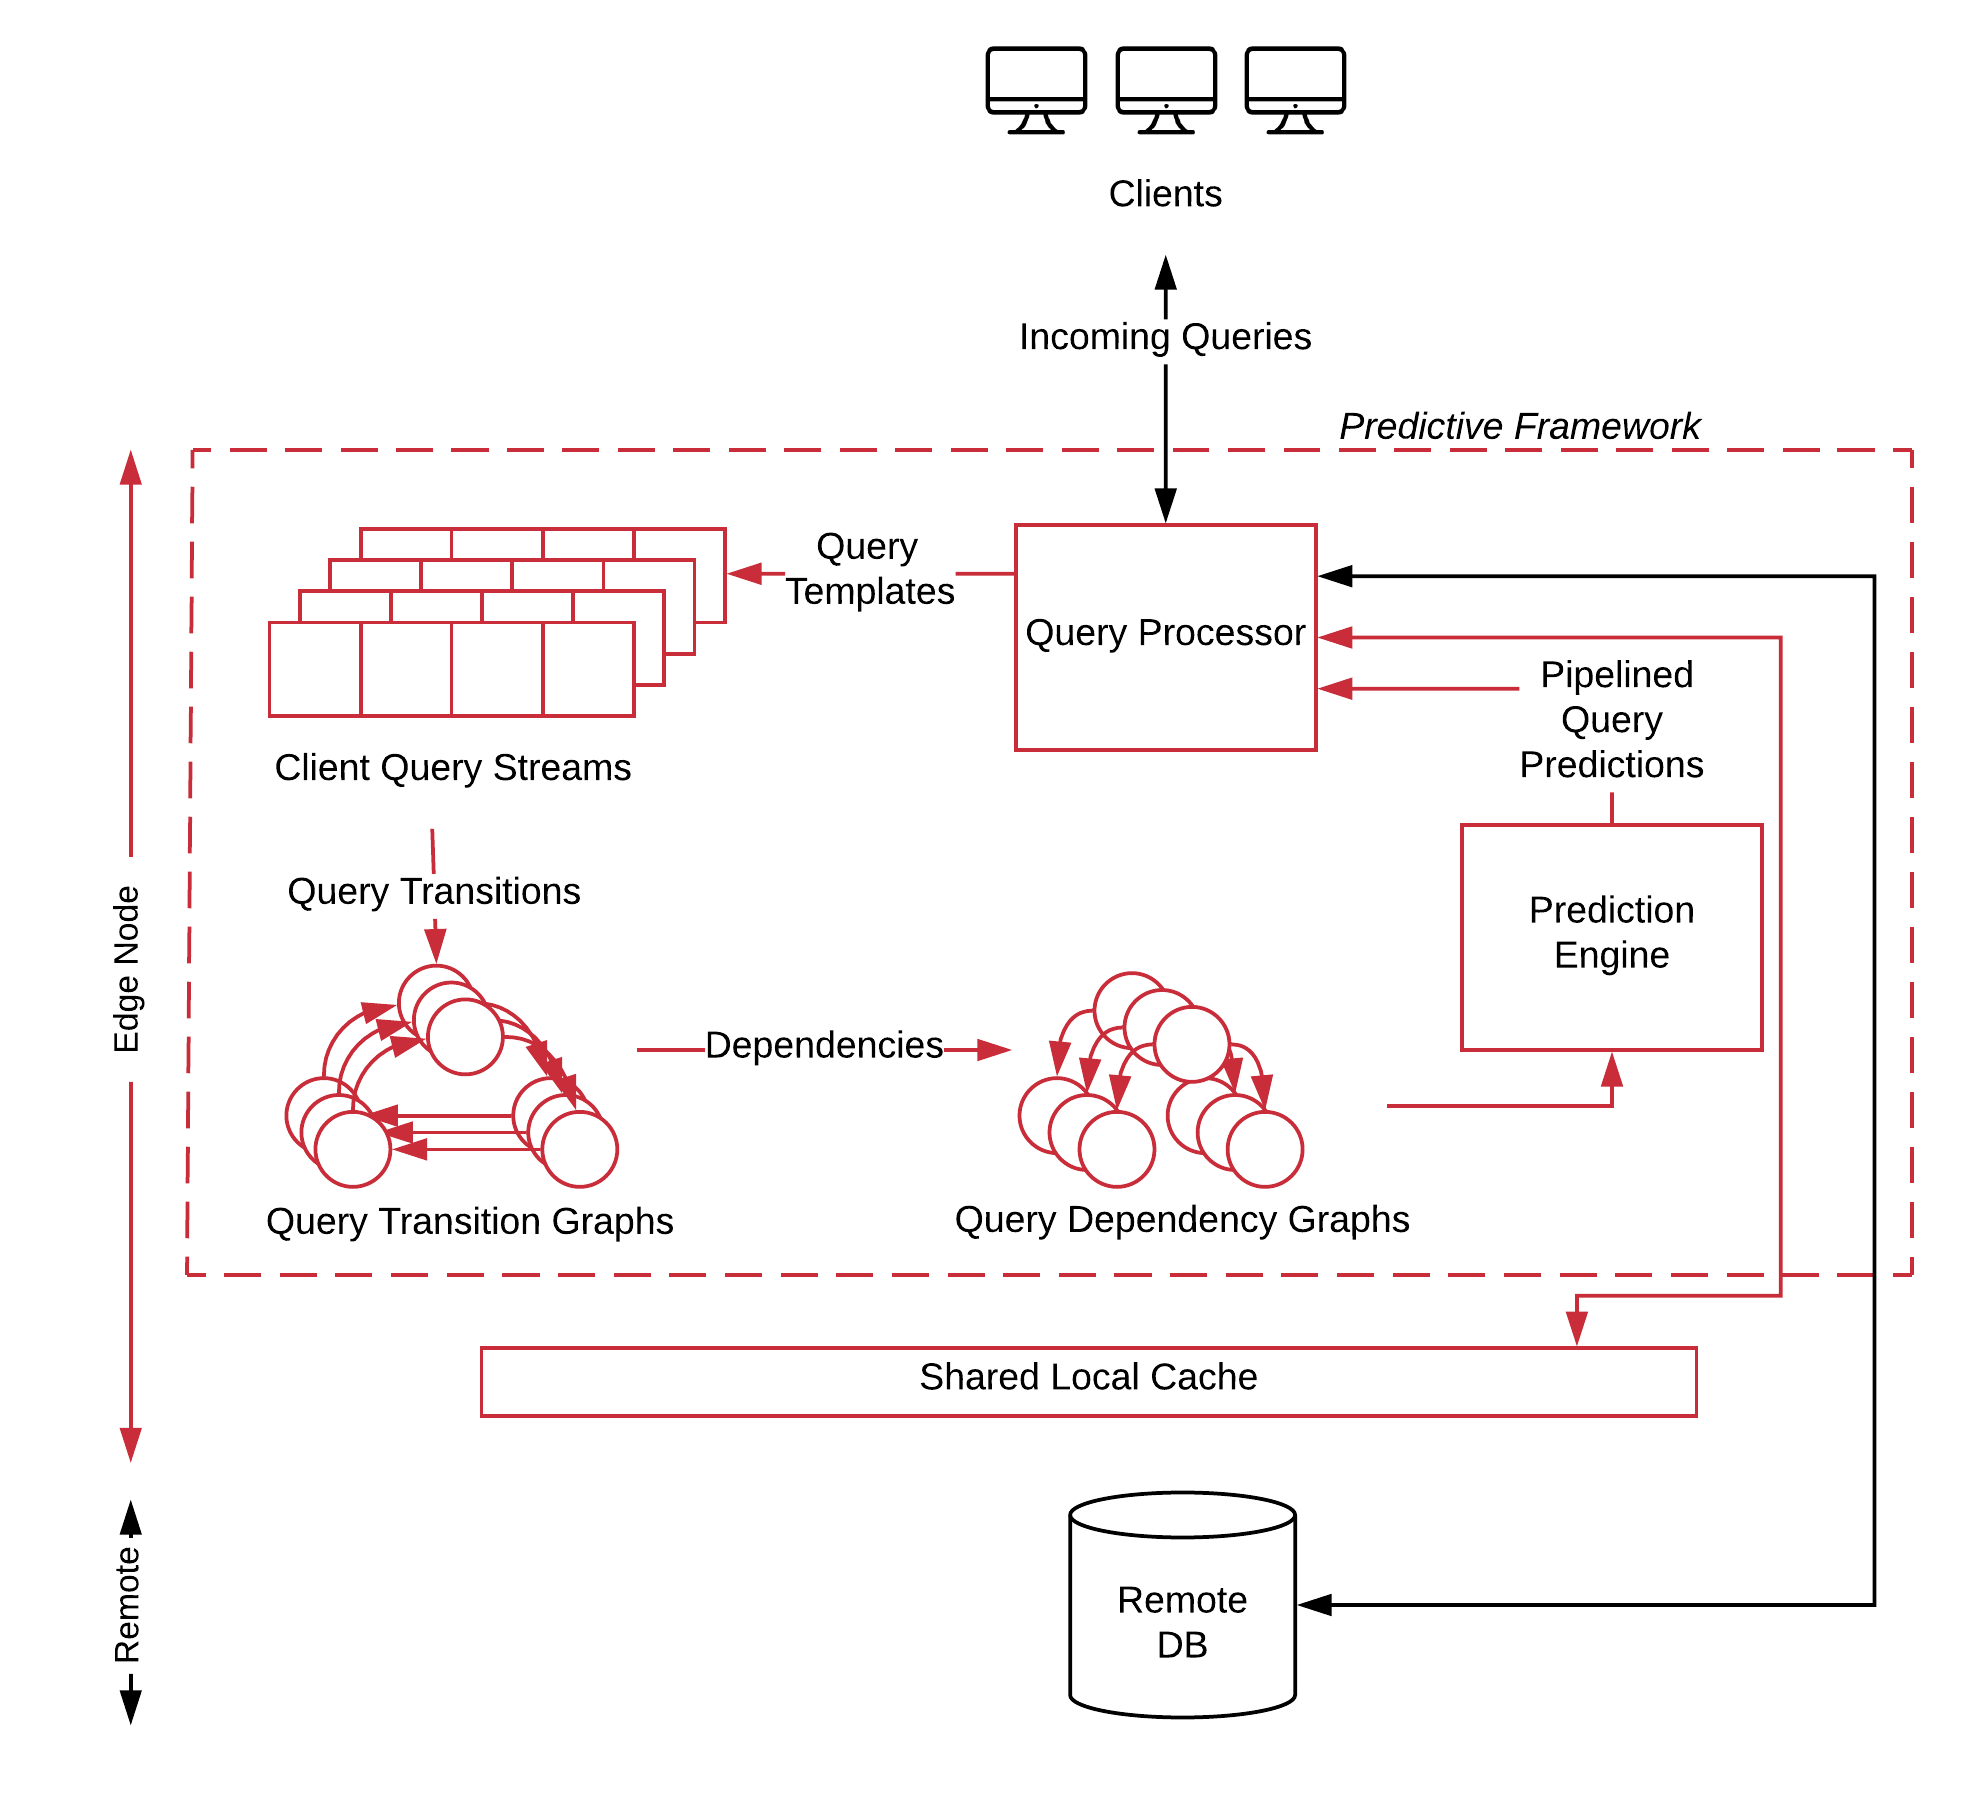
\includegraphics[scale=0.13]{apollo_overview_6}
    \end{figure}
\end{frame}

\begin{frame}[fragile]{Apollo Overview}
    \begin{figure}
        \hspace*{-1cm}
        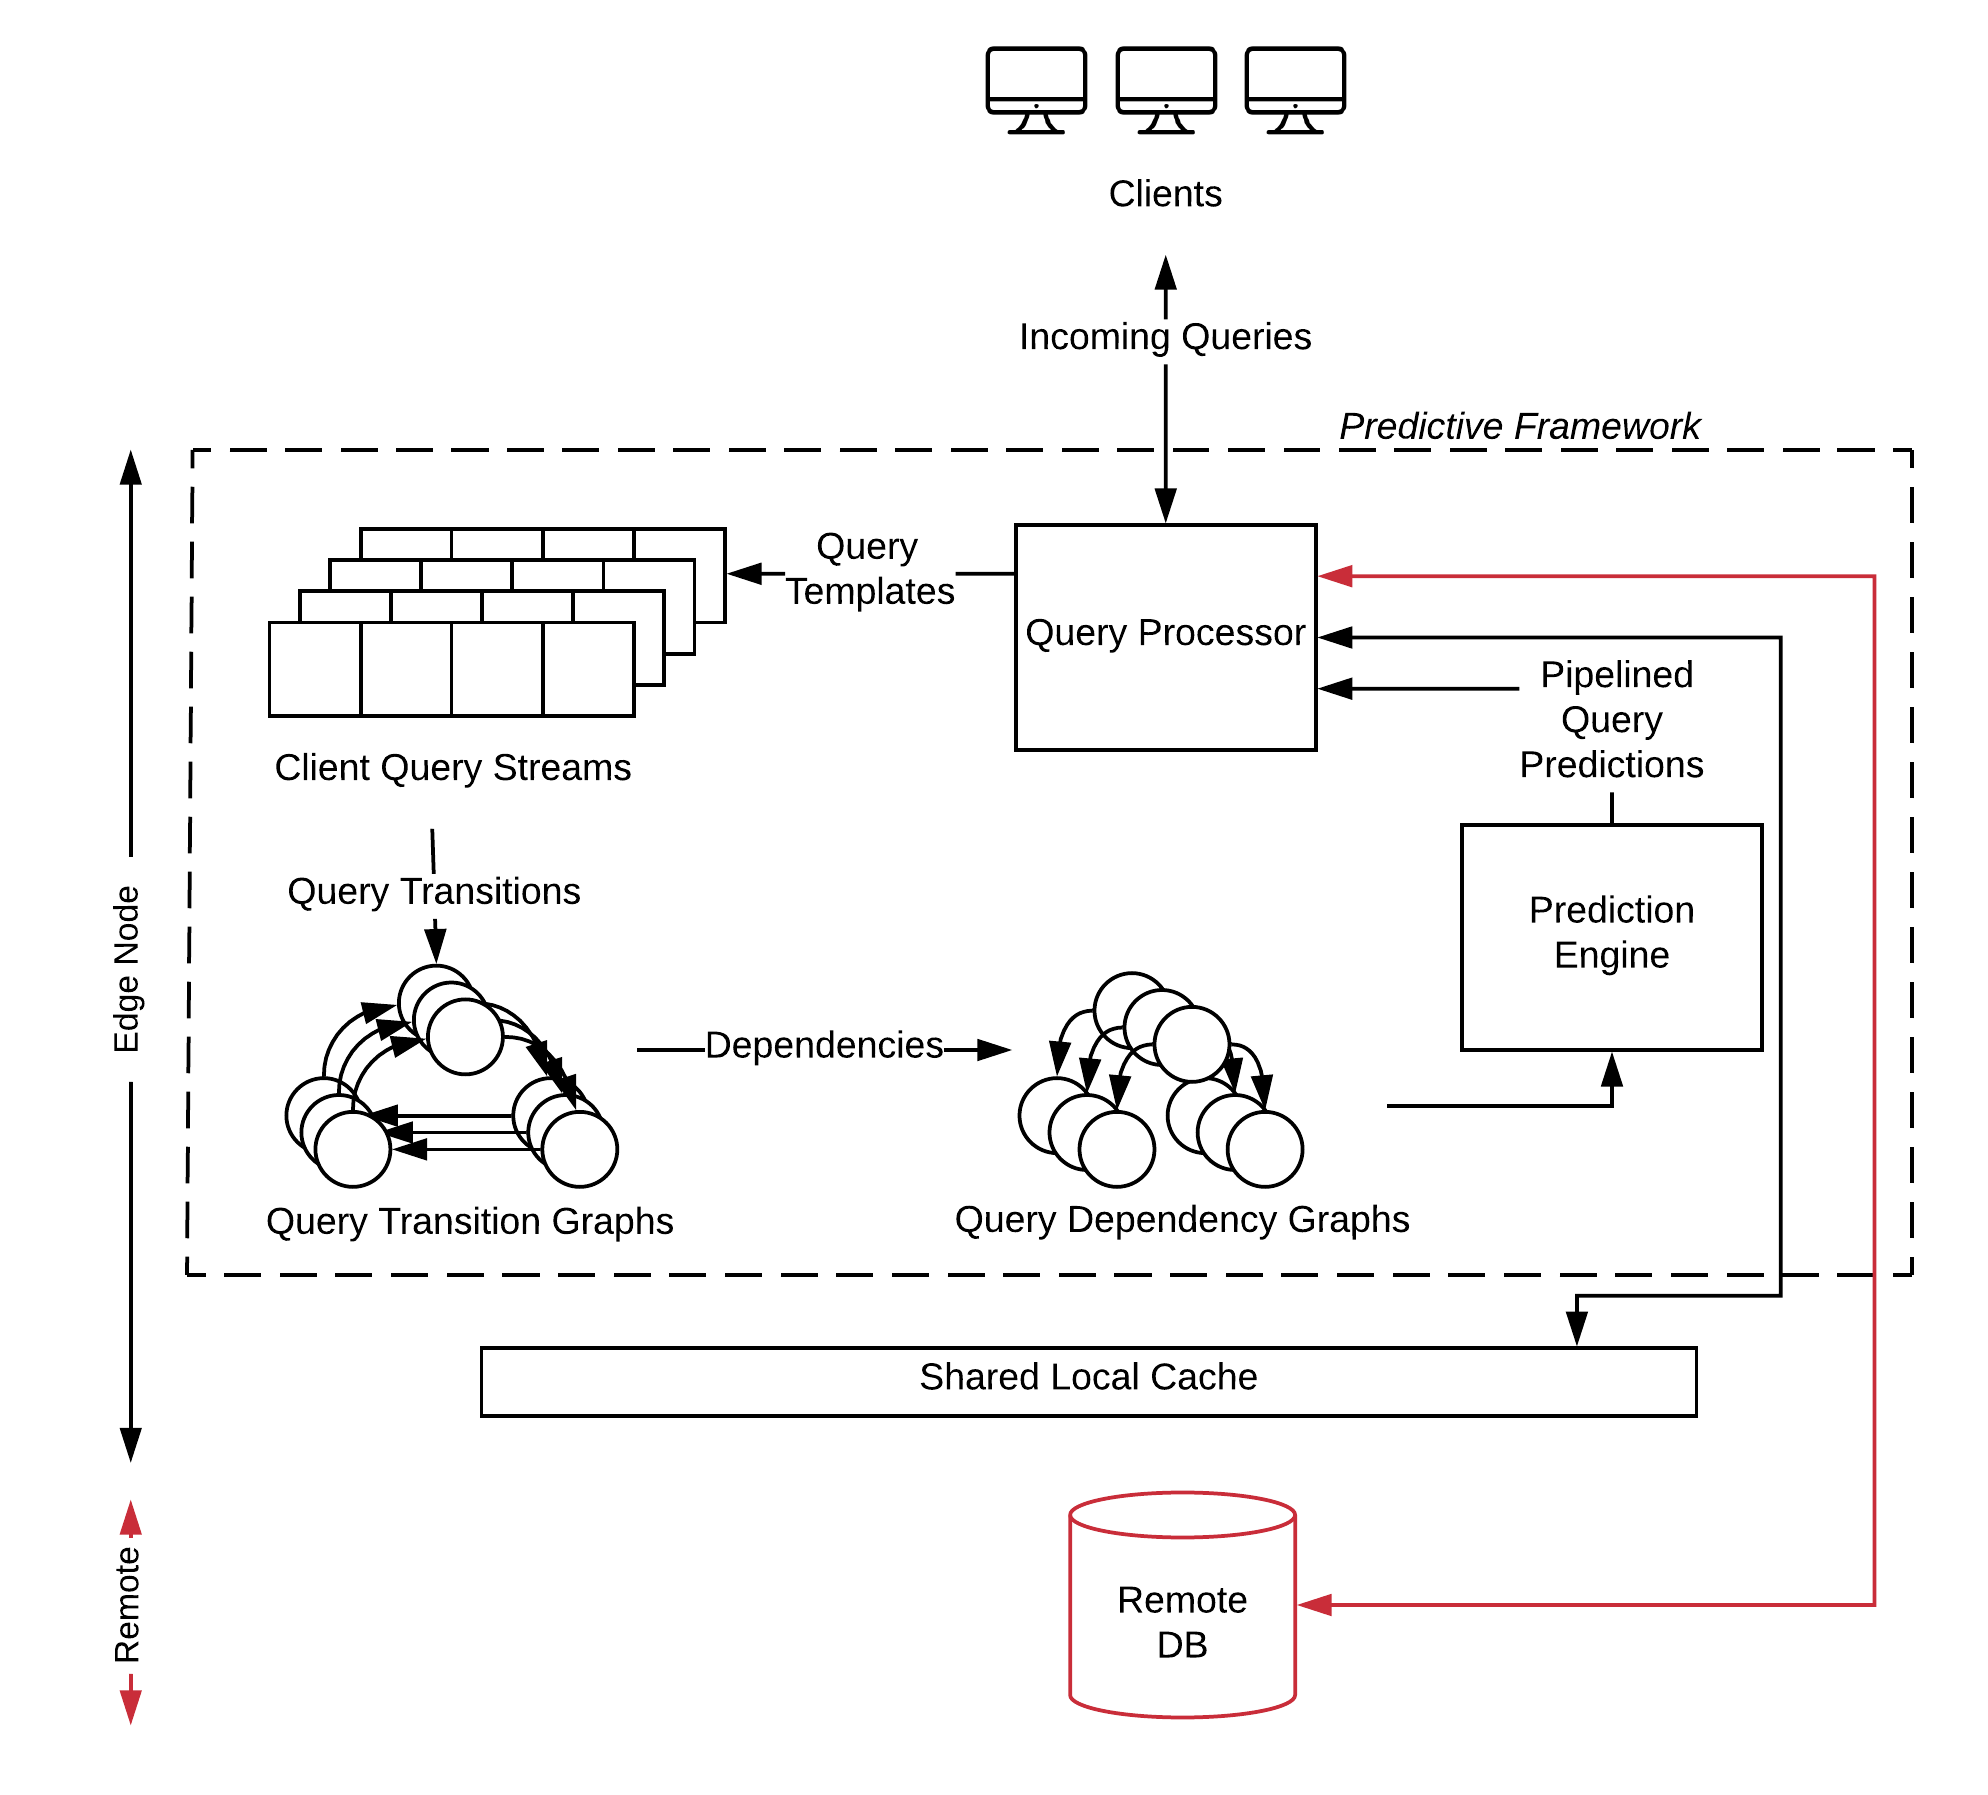
\includegraphics[scale=0.13]{apollo_overview_7}
    \end{figure}
\end{frame}



\begin{frame}[fragile]{A Query Submission}
    \begin{center}
SELECT \cfbox{red}{C\_ID} FROM CUSTOMER WHERE
C\_UNAME = 'Alice' and C\_PASSWD = 'pass'

SELECT MAX(O\_ID) FROM ORDERS WHERE
O\_C\_ID = \cfbox{red}{3}
    \end{center}
\end{frame}


\begin{frame}[fragile]{Query Templates}
    Two query instances, $Q_1$, $Q_2$ share the same \alert{query template} if they have the same
    query text modulo \emph{parameterizable constants}.
\end{frame}

\begin{frame}[fragile]{Abstracting Query Instances to Query Templates}
    \begin{center}
SELECT \cfbox{red}{C\_ID} FROM CUSTOMER WHERE
C\_UNAME = \textbf{?} and C\_PASSWD = \textbf{?}

SELECT MAX(O\_ID) FROM ORDERS WHERE
O\_C\_ID = \cfbox{red}{\textbf{?}}
    \end{center}
\end{frame}


\begin{frame}[fragile]{Client Query Streams}
    \begin{figure}
        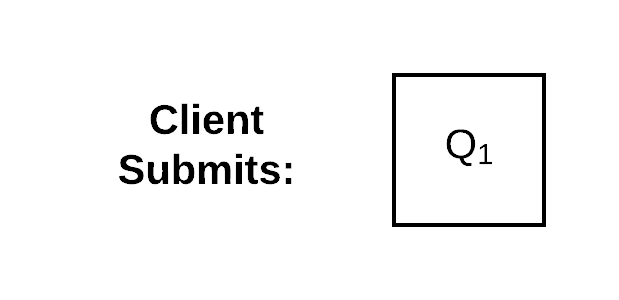
\includegraphics[scale=0.2]{apollo_client_query_stream_0}
    \end{figure}
\end{frame}

\begin{frame}[fragile]{Client Query Streams}
    \begin{figure}
        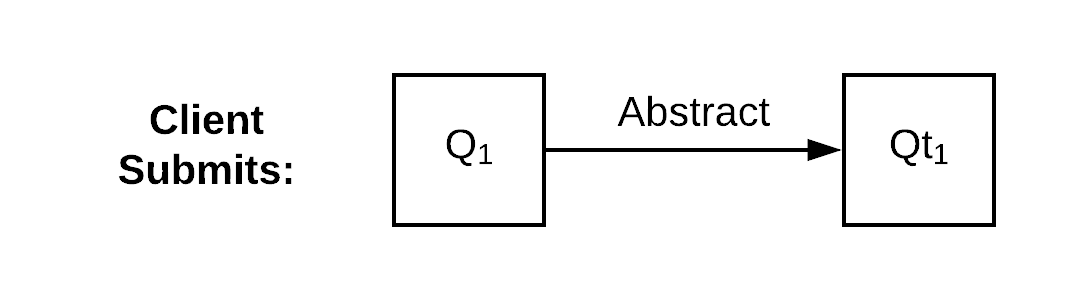
\includegraphics[scale=0.2]{apollo_client_query_stream_0_2}
    \end{figure}

\end{frame}

\begin{frame}[fragile]{Client Query Streams}
    \begin{figure}
        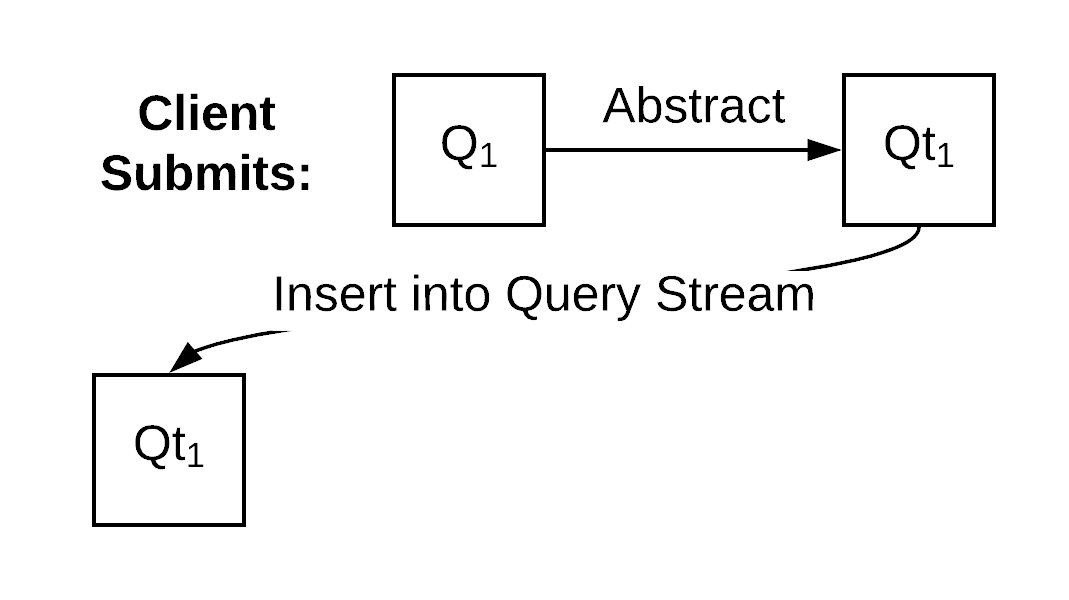
\includegraphics[scale=0.2]{apollo_client_query_stream_0_3}
    \end{figure}
\end{frame}

\begin{frame}[fragile]{Client Query Streams}
    \begin{figure}
        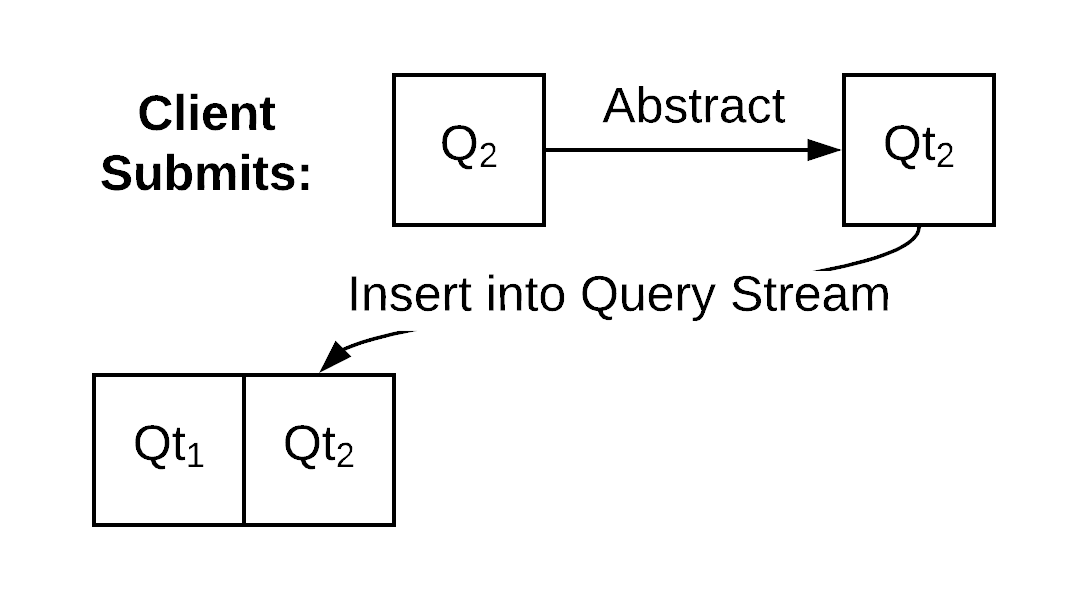
\includegraphics[scale=0.2]{apollo_client_query_stream_0_4}
    \end{figure}
\end{frame}

\begin{frame}[fragile]{Client Query Streams}
    \begin{figure}
        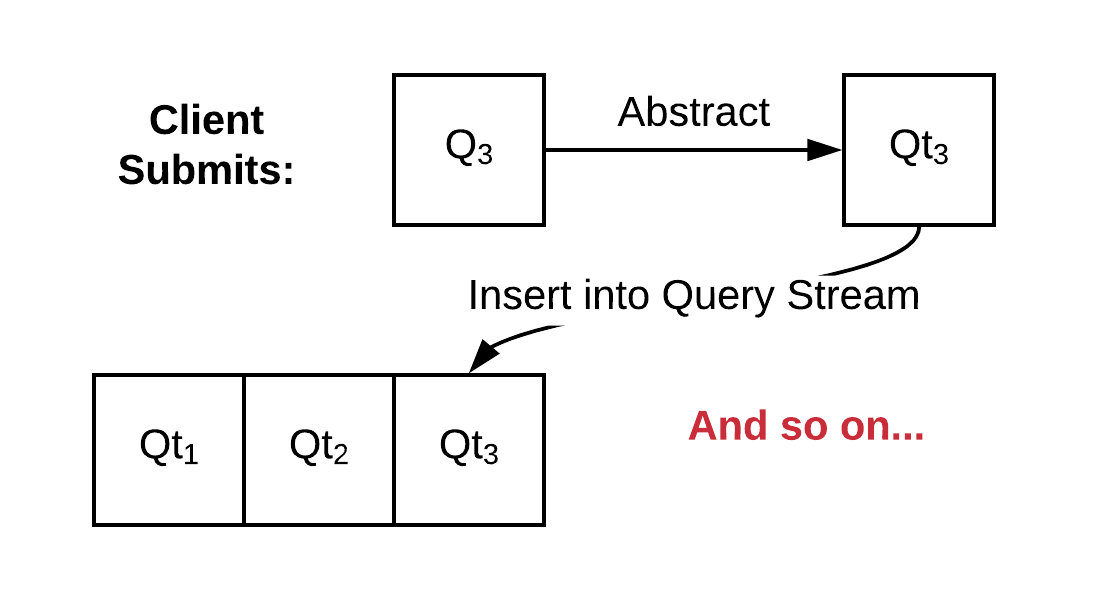
\includegraphics[scale=0.2]{apollo_client_query_stream_0_5}
    \end{figure}
\end{frame}

\begin{frame}[fragile]{Client Query Streams}
    \begin{figure}
        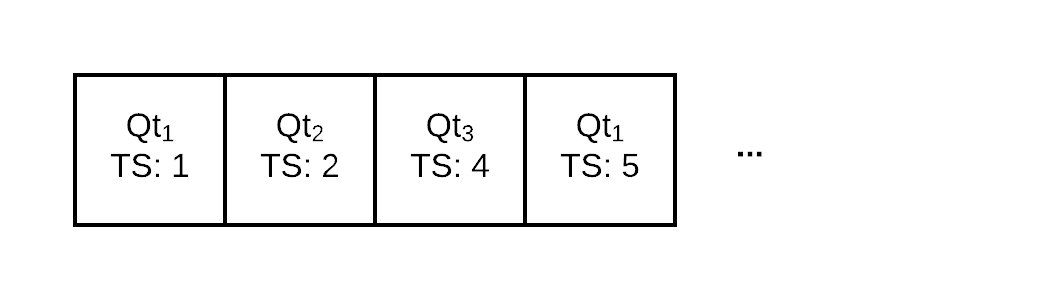
\includegraphics[scale=0.2]{apollo_client_query_stream}
    \end{figure}
\end{frame}

\begin{frame}[fragile]{Client Query Streams}
    \begin{figure}
        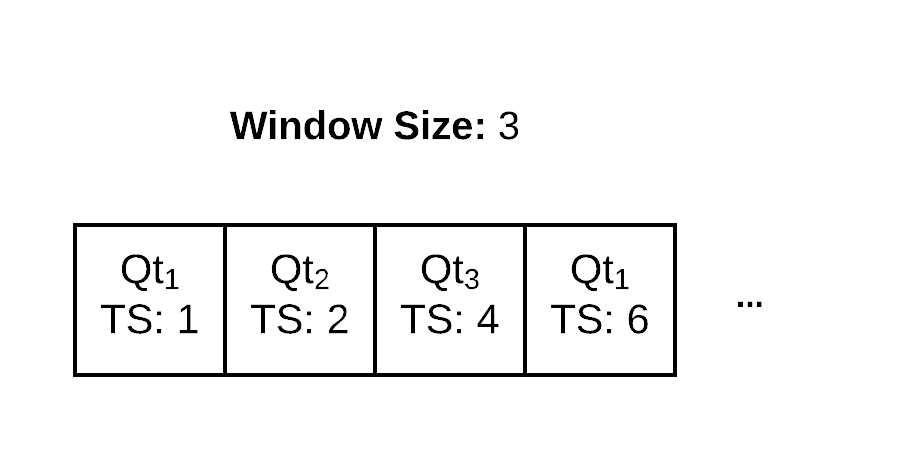
\includegraphics[scale=0.2]{apollo_client_query_stream_2}
    \end{figure}
\end{frame}

\begin{frame}[fragile]{Client Query Streams}
    \begin{figure}
        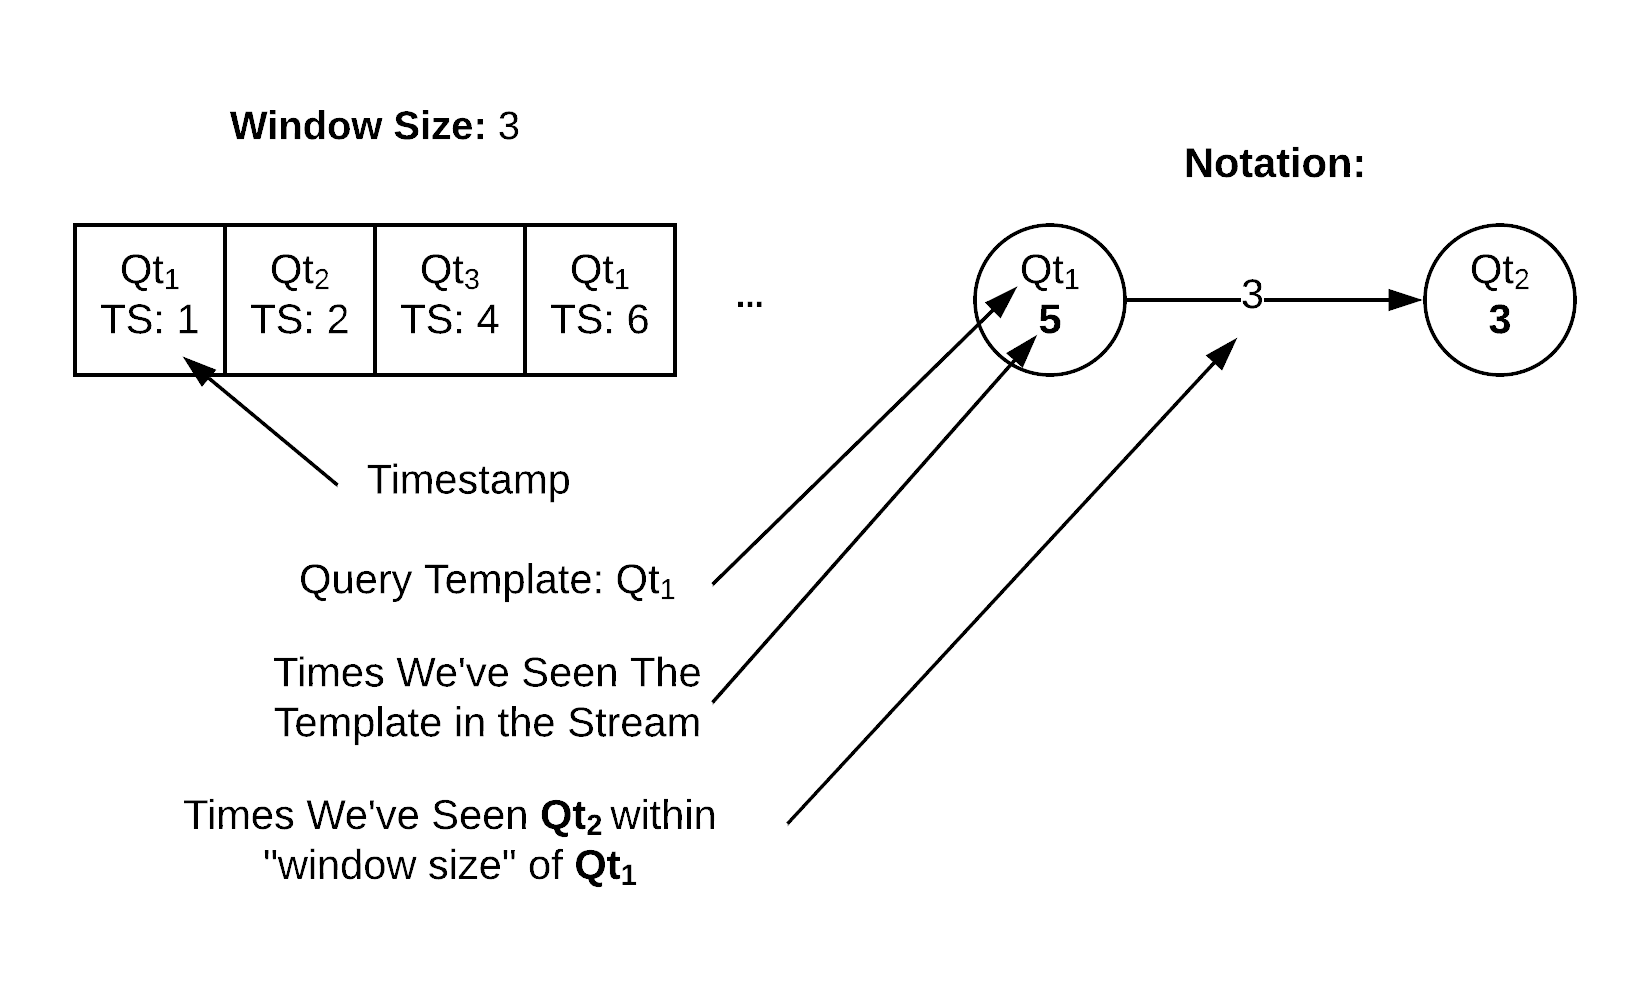
\includegraphics[scale=0.2]{apollo_client_query_stream_2_1}
    \end{figure}
\end{frame}



\begin{frame}[fragile]{Client Query Streams}
    \begin{figure}
        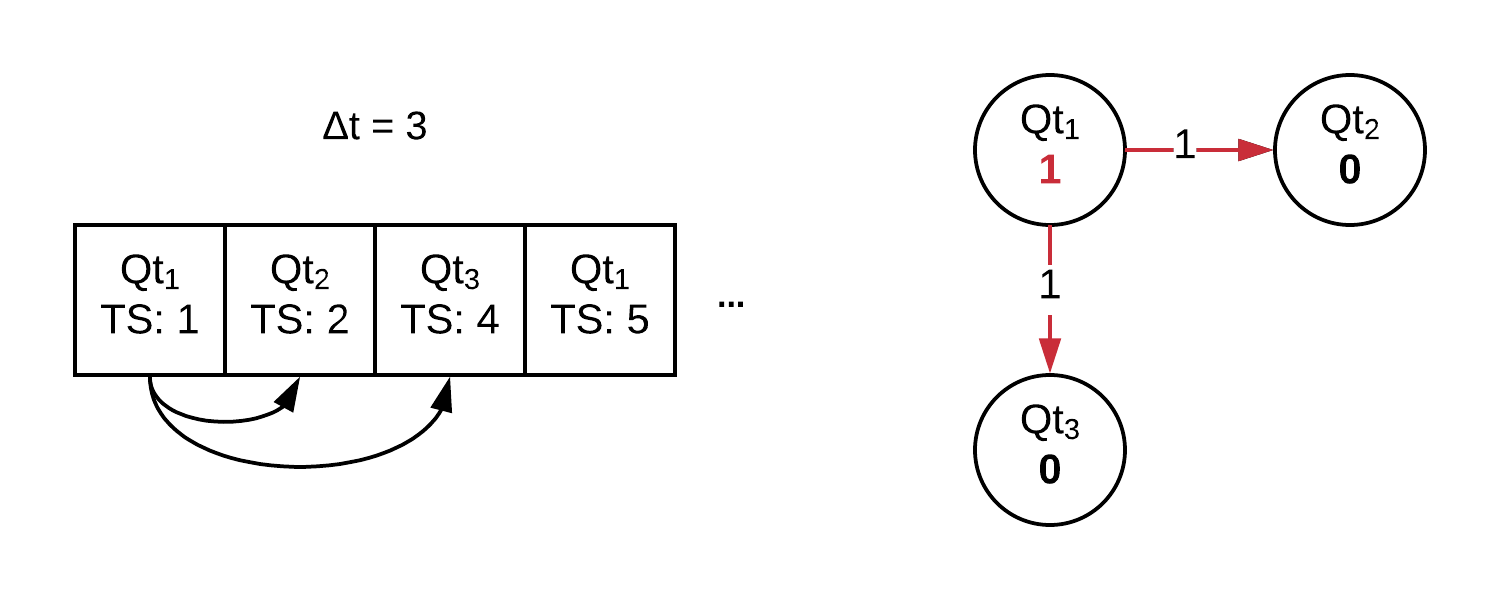
\includegraphics[scale=0.2]{apollo_client_query_stream_3}
    \end{figure}
\end{frame}

\begin{frame}[fragile]{Client Query Streams}
    \begin{figure}
        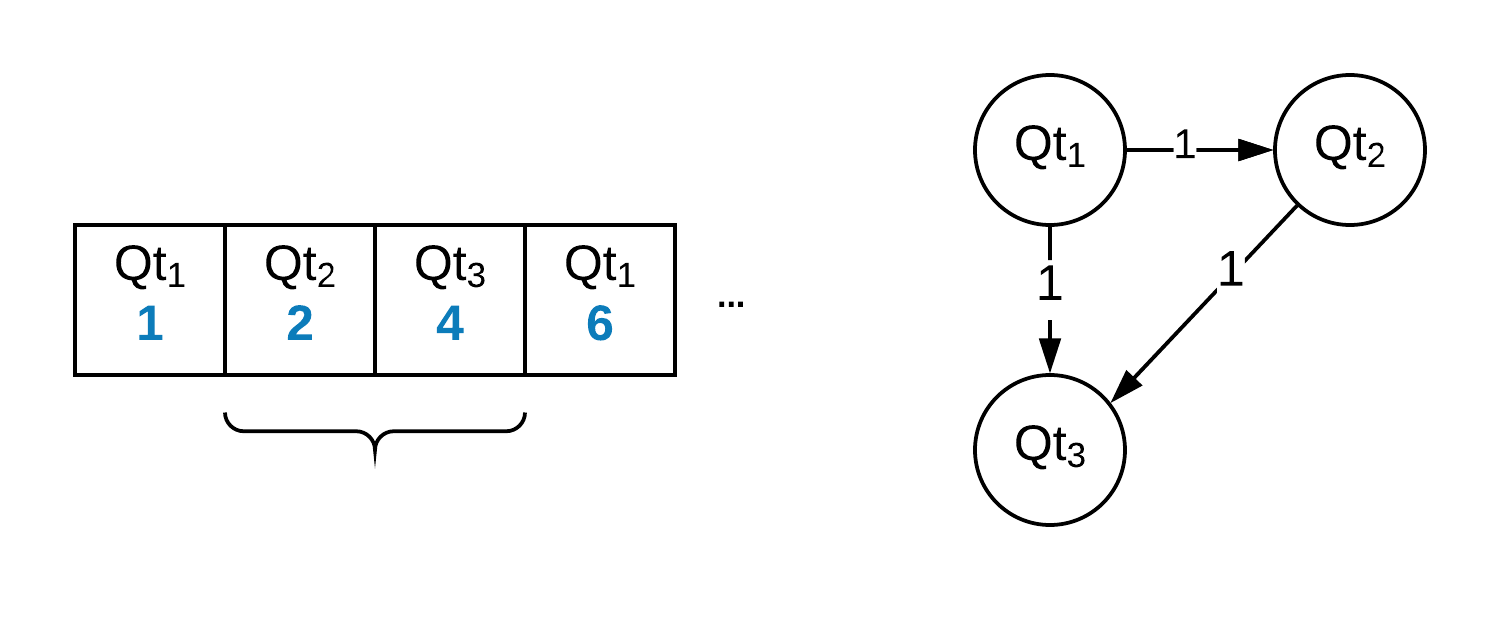
\includegraphics[scale=0.2]{apollo_client_query_stream_4}
    \end{figure}
\end{frame}

\begin{frame}[fragile]{Client Query Streams}
    \begin{figure}
        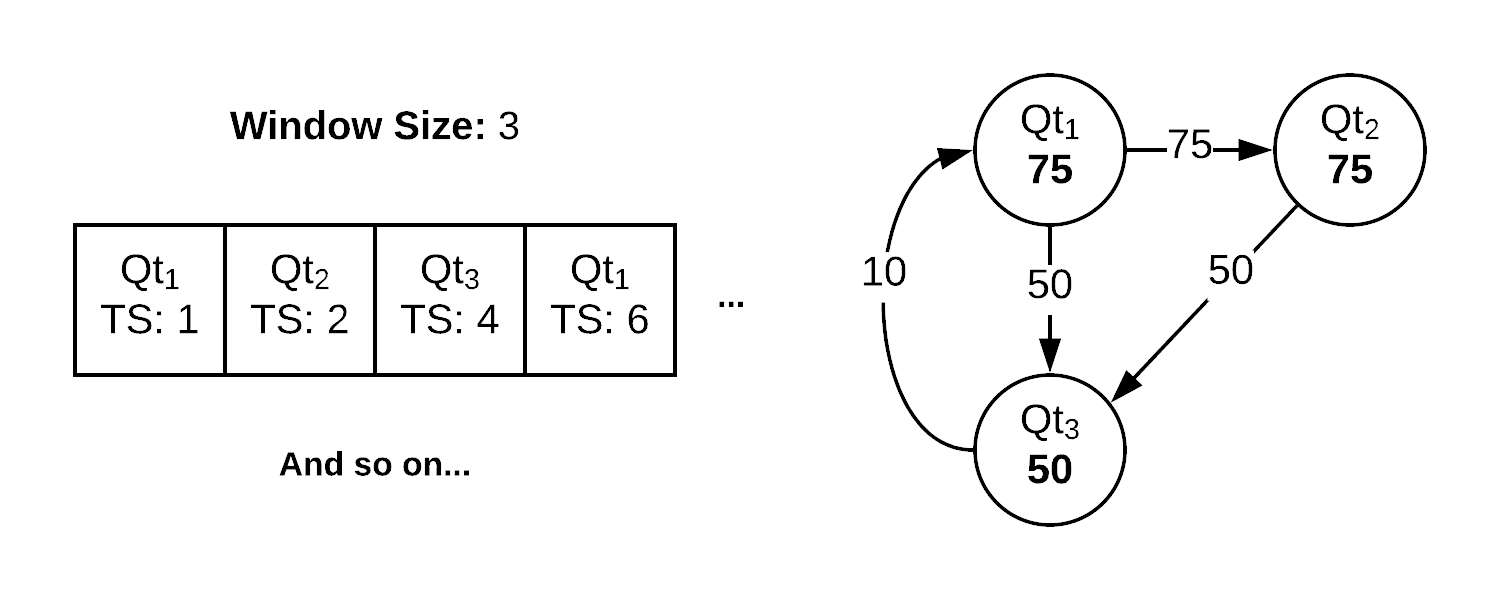
\includegraphics[scale=0.2]{apollo_client_query_stream_5}
    \end{figure}
\end{frame}

\begin{frame}[fragile]{Query Transition Graph}
    \begin{figure}
        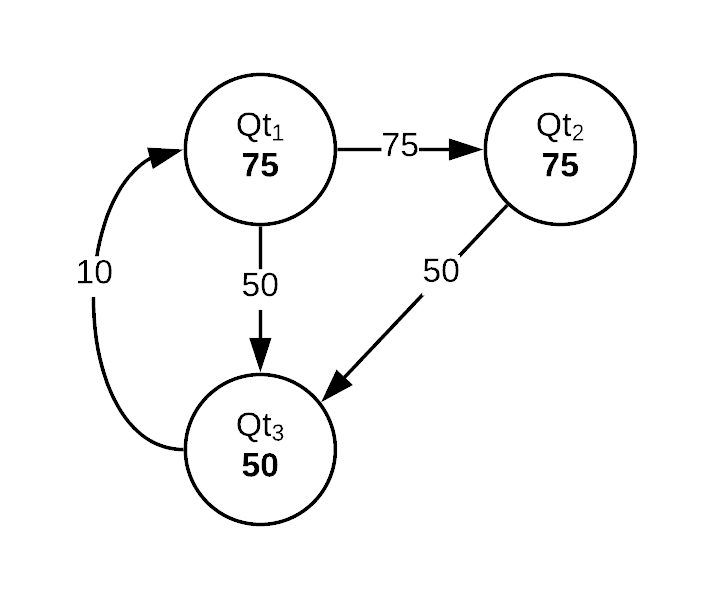
\includegraphics[scale=0.2]{apollo_transition_graph}
    \end{figure}
    \visible<2->{
        Probability of seeing $Qt_{2}$ within sliding window after we've seen $Qt_{1}$:\\
        $P(Qt_{2}|Qt_{1};T\leq\Delta t) = \frac{\textrm{times } Qt_{2} \textrm{ executed within window of } Qt_{1}}{\textrm{times } Qt_{1} \textrm{ executed}} =\frac{75}{75} = 1$\\
    }
    \visible<3->{
        $P(Qt_{3}|Qt_{1};T\leq\Delta t) = \frac{10}{50} = \frac{1}{5}$
    }
\end{frame}

\begin{frame}[fragile]{Query Transition Graph}
    The query transition graphs tells us:
    \begin{itemize}
        \item{How often a query template is executed}
        \visible<2->{
        \item{Which query templates are \alert{correlated} with each other. If correlation is sufficiently high ($>$ correlation threshold), then we
        monitor input and output sets for the queries.}
        }
    \end{itemize}
    \visible<3->{
        { \color{red} Need parameter mappings for predictive caching!}
    }
\end{frame}

\begin{frame}[fragile]{Client Query Streams}
    \begin{figure}
        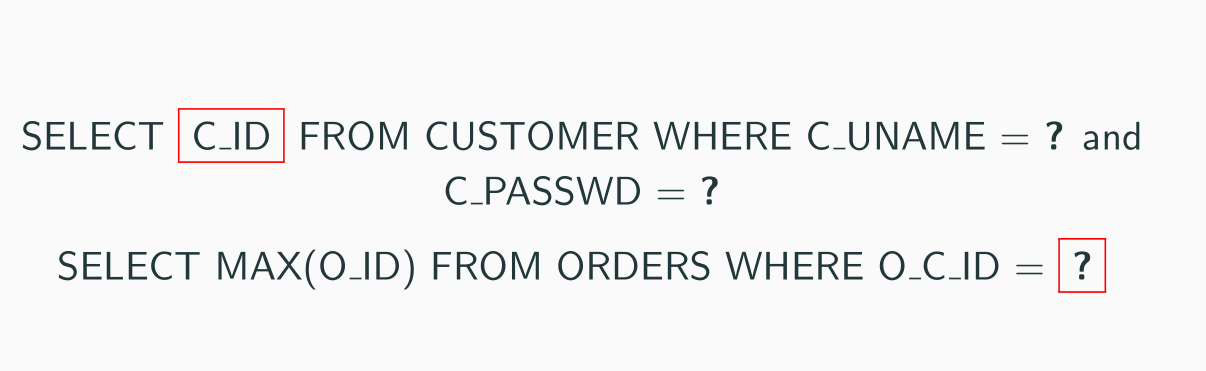
\includegraphics[scale=0.25]{apollo_parameter_mappings}
    \end{figure}
\end{frame}

\begin{frame}[fragile]{Client Query Streams}
    \begin{figure}
        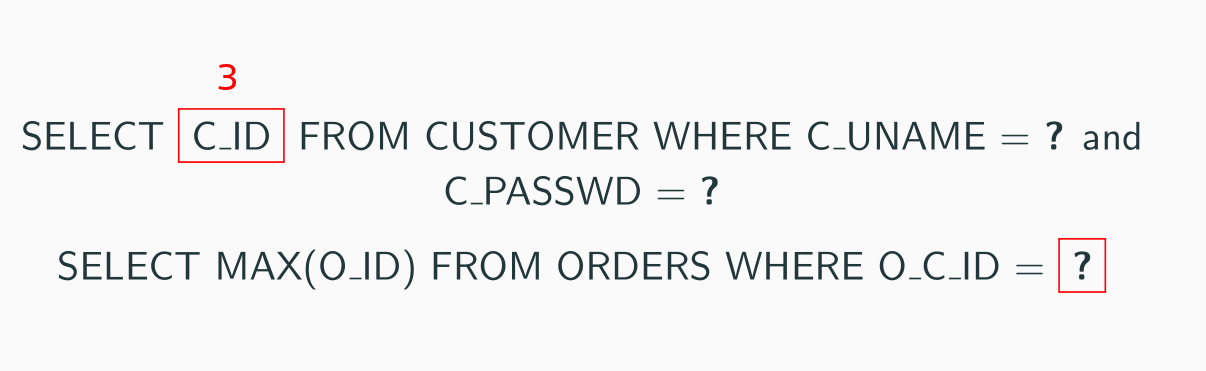
\includegraphics[scale=0.25]{apollo_parameter_mappings_2}
    \end{figure}
\end{frame}

\begin{frame}[fragile]{Client Query Streams}
    \begin{figure}
        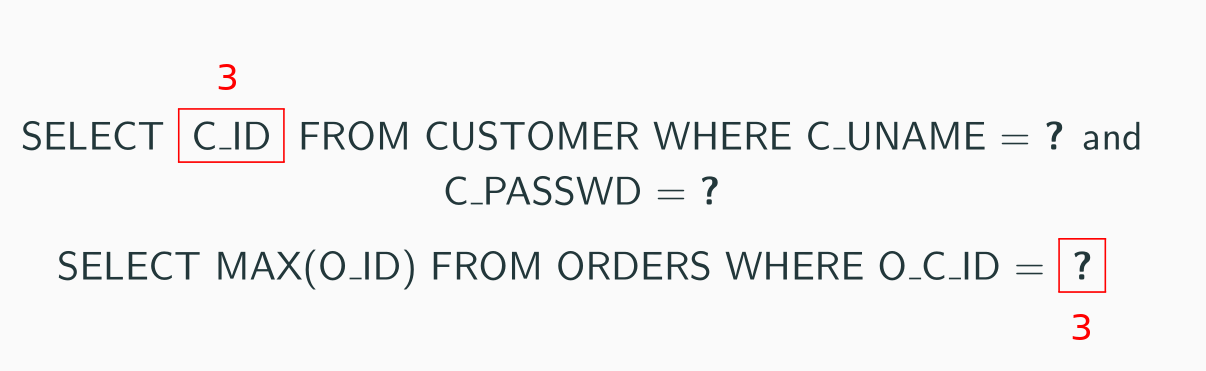
\includegraphics[scale=0.25]{apollo_parameter_mappings_3}
    \end{figure}
\end{frame}

\begin{frame}[fragile]{Client Query Streams}
    \begin{figure}
        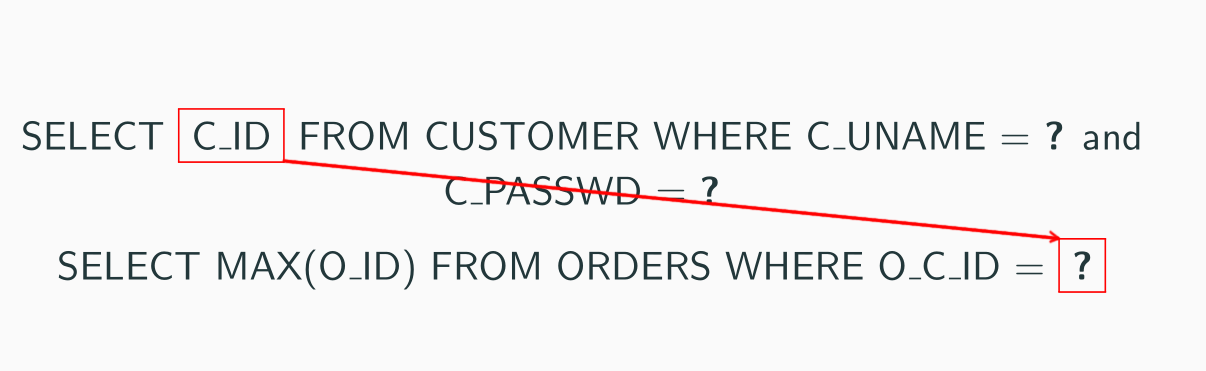
\includegraphics[scale=0.25]{apollo_parameter_mappings_4}
    \end{figure}
\end{frame}

\begin{frame}[fragile]{Query Dependency Graph}
    \begin{figure}
        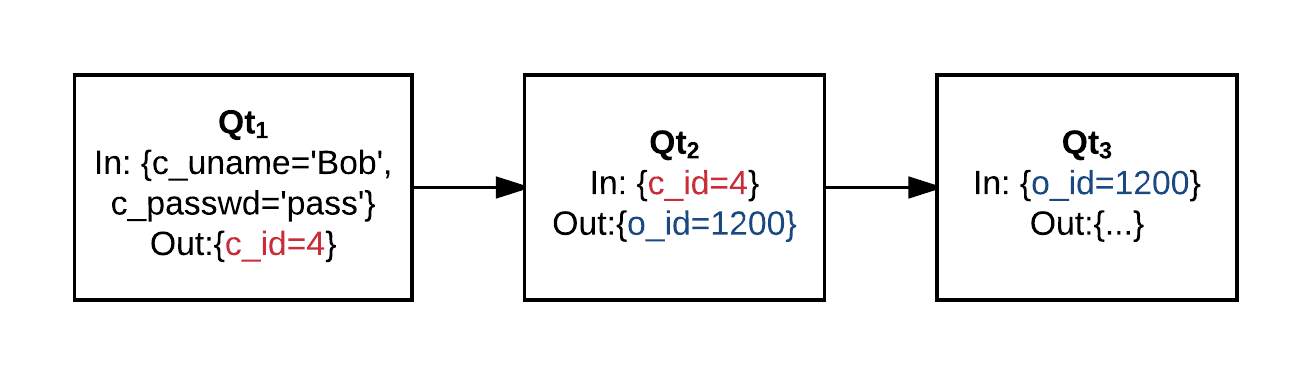
\includegraphics[scale=0.22]{apollo_query_pipeline}
    \end{figure}
\end{frame}

\begin{comment}
\begin{frame}[fragile]{Fully Defined Queries}
A \alert{fully defined query template} (FDQ) $\mathit{Qt}_j$ has all of its inputs provided
by some set, possibly empty, of prior query templates $\mathit{Qt_i}_1, \mathit{Qt_i}_2, \ldots, \mathit{Qt_i}_m$.
\end{frame}

\begin{frame}[fragile]{Example FDQs}
    \begin{figure}
        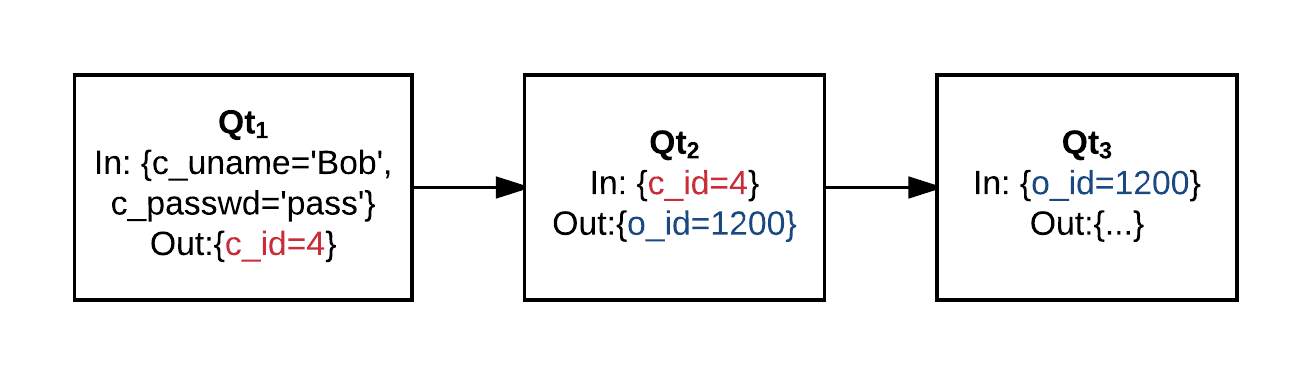
\includegraphics[scale=0.22]{apollo_query_pipeline}
    \end{figure}
    \visible<2->{
        $\mathit{Qt}_2$ and $\mathit{Qt}_3$ are FDQs.\\
    }
    \visible<3->{
        $\mathit{Qt}_1$ is a dependency query of $\mathit{Qt}_2$.\\
        $\mathit{Qt}_2$ is a dependency query of $\mathit{Qt}_3$.\\
    }
\end{frame}

\end{comment}

\begin{frame}[fragile]{Core Prediction Routine}
    \begin{figure}
        \hspace*{-1cm}
        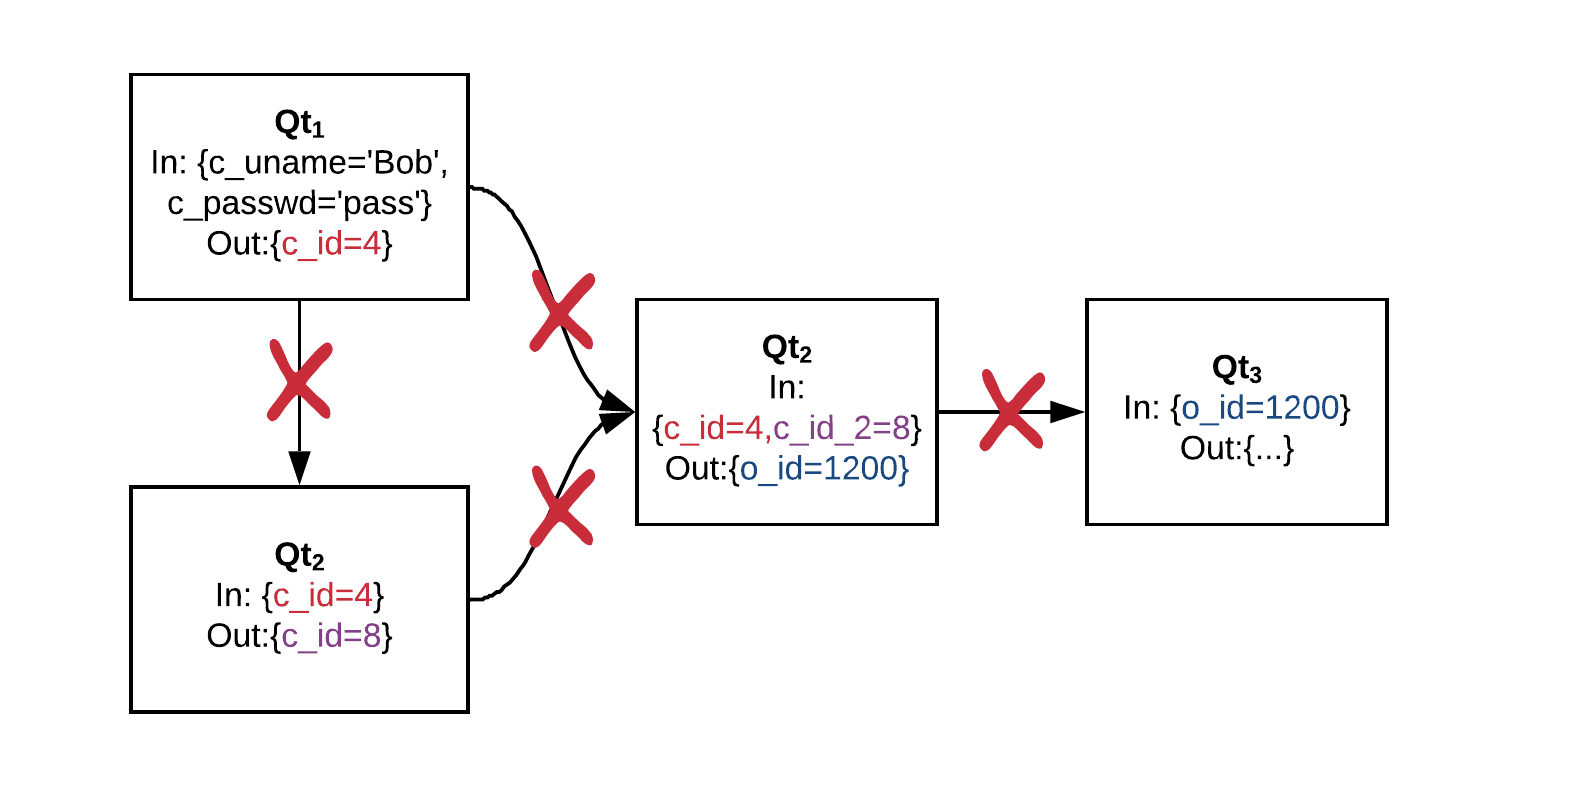
\includegraphics[scale=0.22]{apollo_cpr}
    \end{figure}
\end{frame}

\begin{frame}[fragile]{Core Prediction Routine}
    \begin{figure}
        \hspace*{-1cm}
        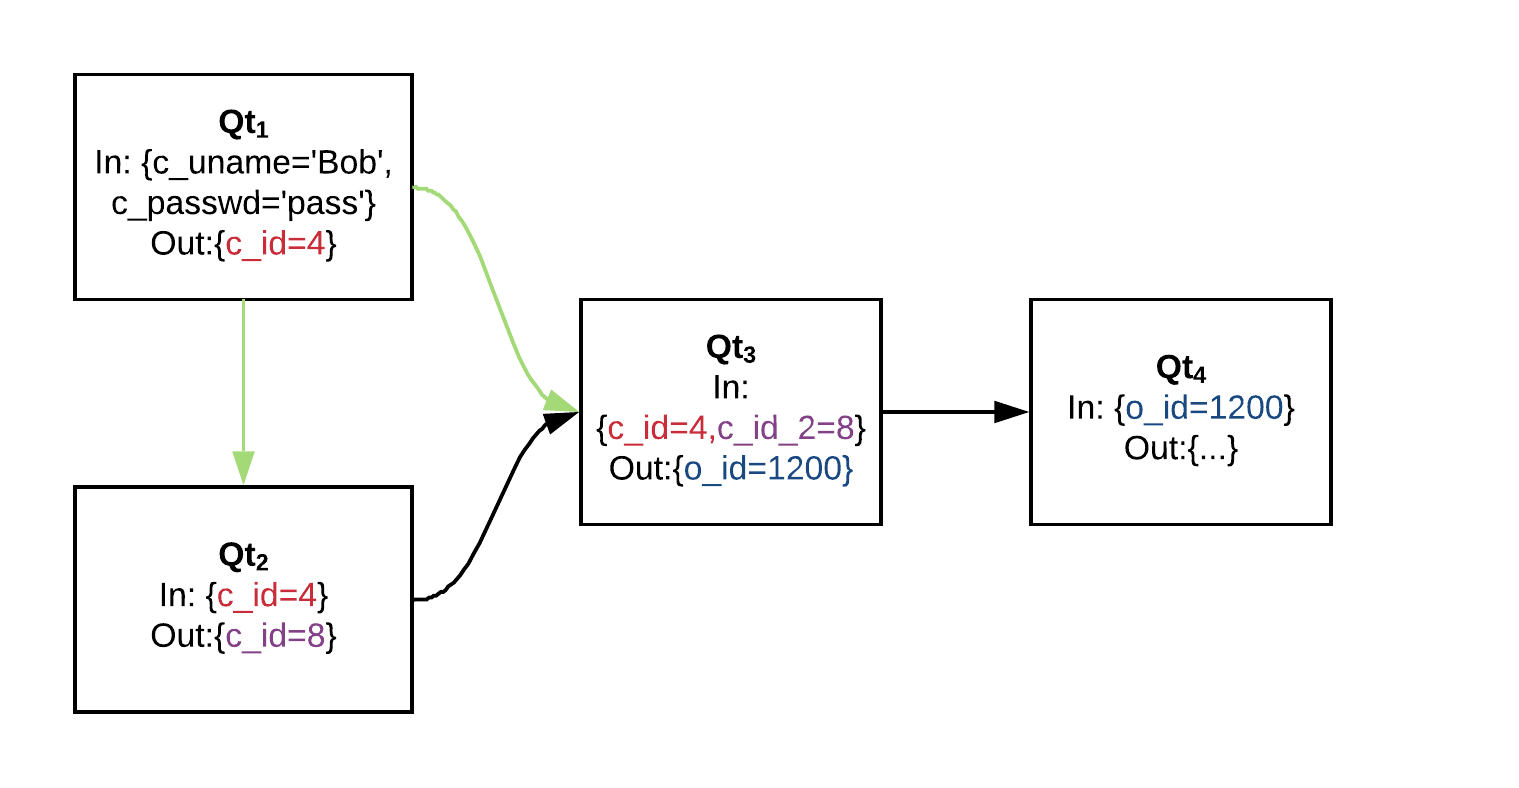
\includegraphics[scale=0.22]{apollo_cpr_2}
    \end{figure}
\end{frame}

\begin{frame}[fragile]{Core Prediction Routine}
    \begin{figure}
        \hspace*{-1cm}
        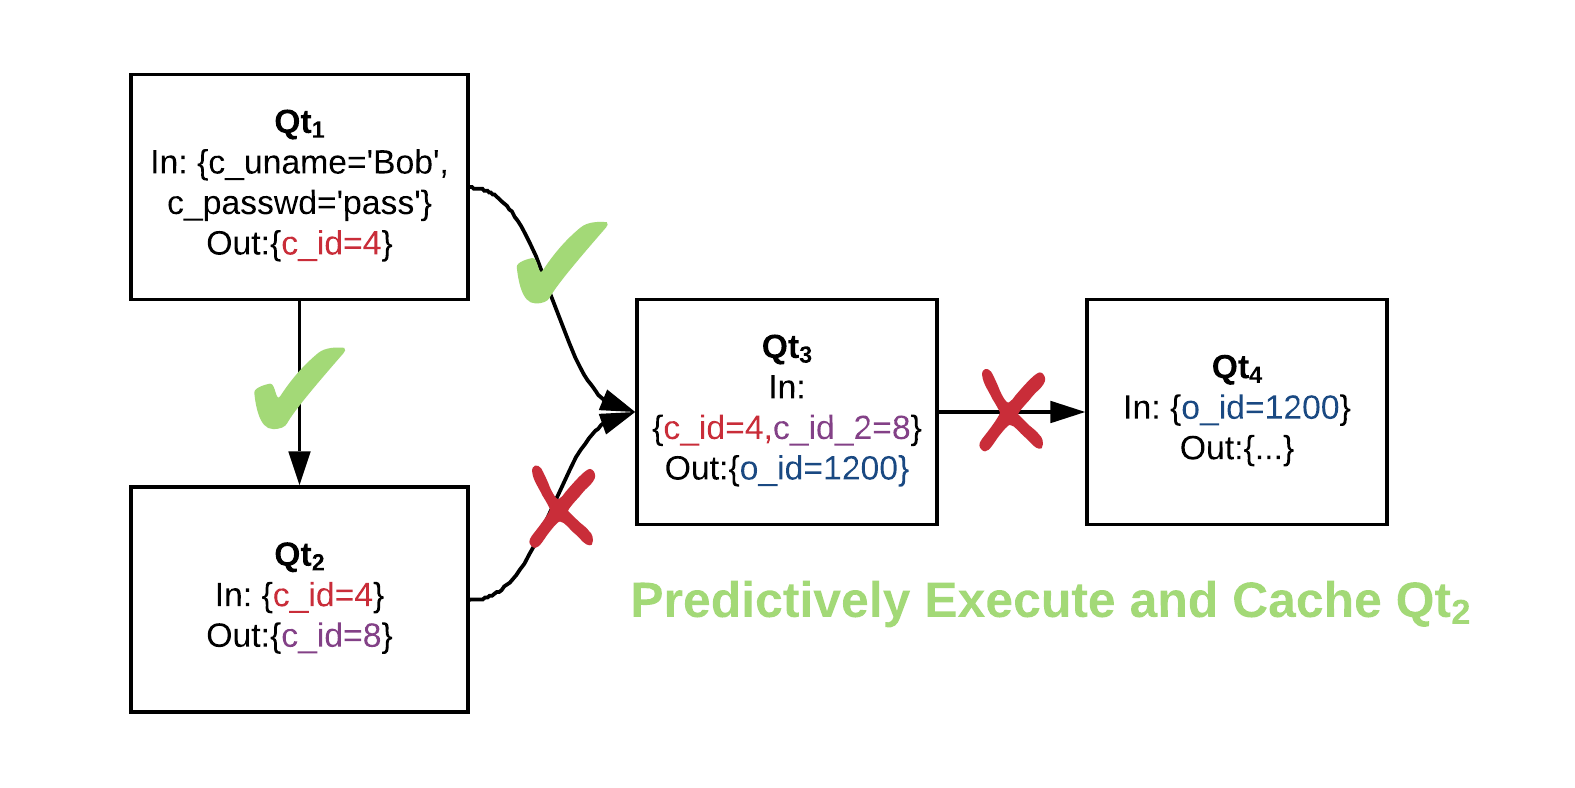
\includegraphics[scale=0.22]{apollo_cpr_3}
    \end{figure}
\end{frame}

\begin{frame}[fragile]{Core Prediction Routine}
    \begin{figure}
        \hspace*{-1cm}
        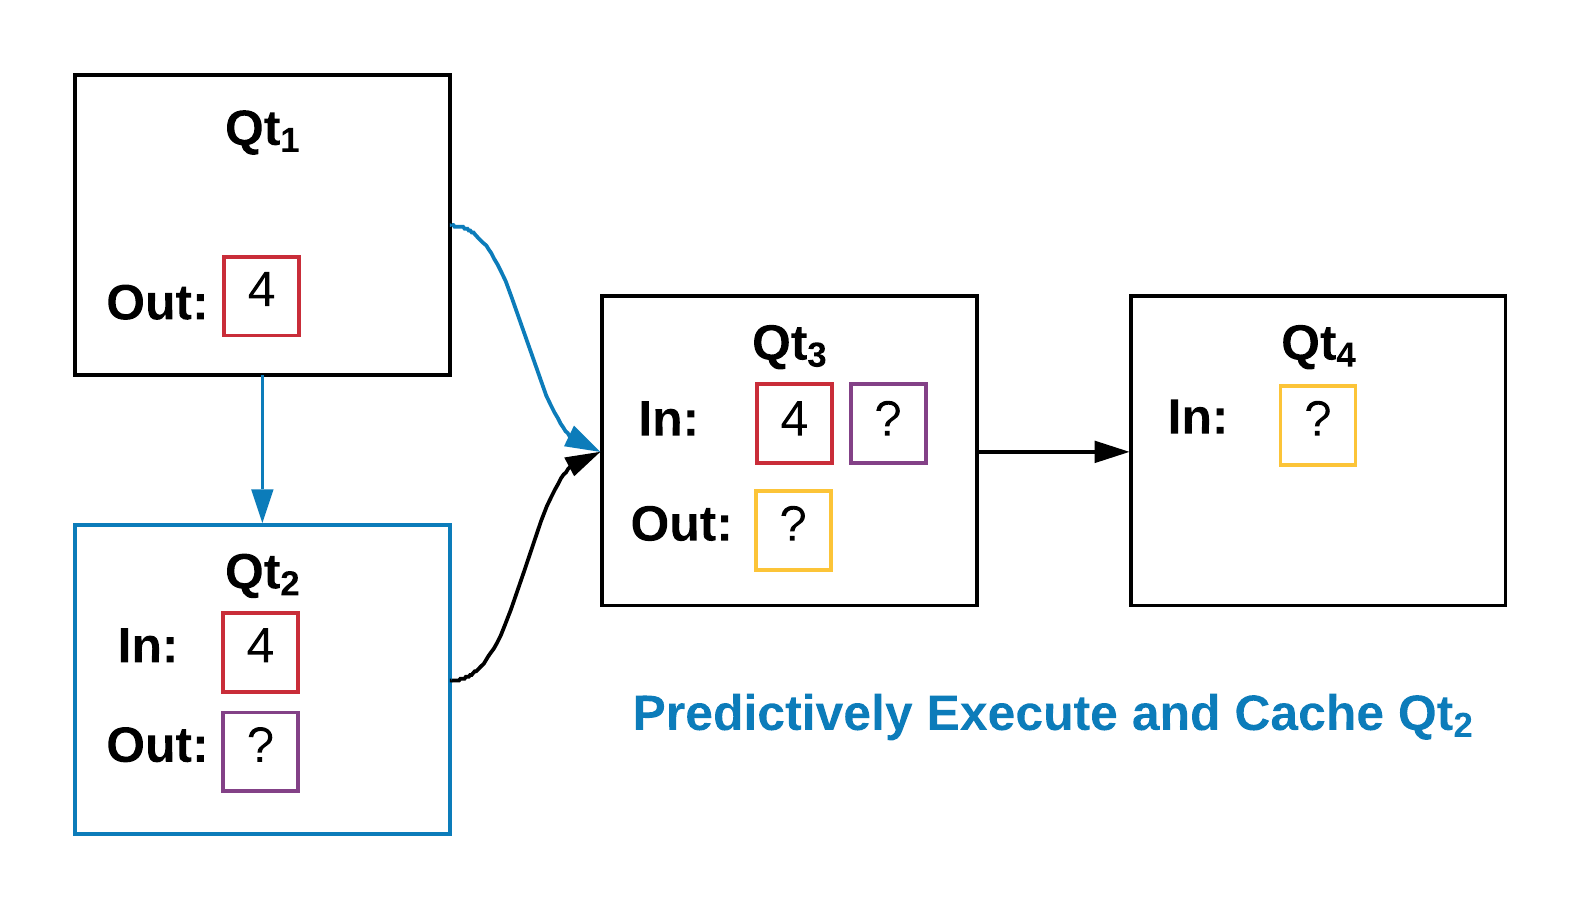
\includegraphics[scale=0.22]{apollo_cpr_4}
    \end{figure}
\end{frame}

\begin{frame}[fragile]{Core Prediction Routine}
    \begin{figure}
        \hspace*{-1cm}
        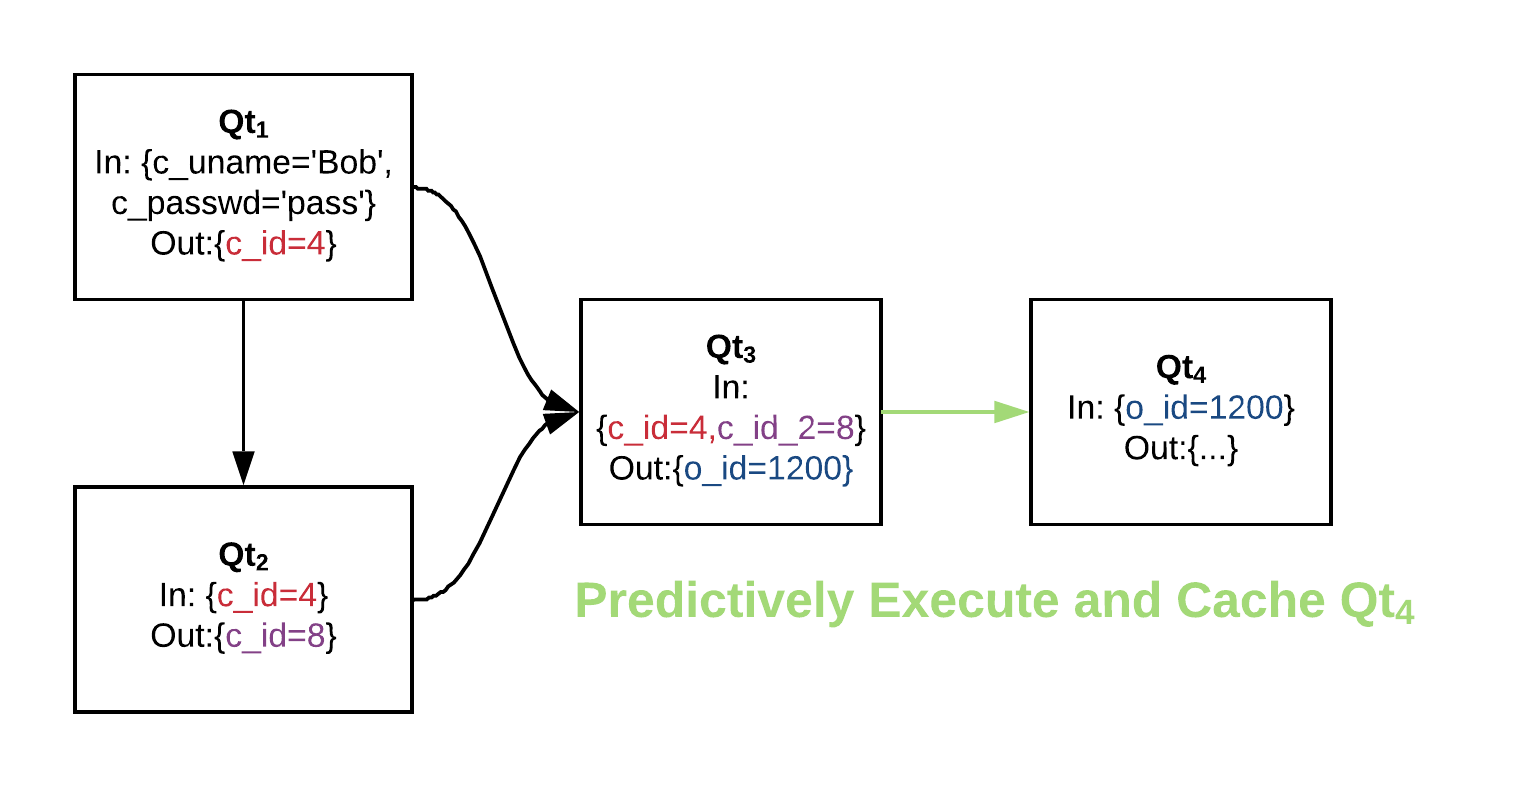
\includegraphics[scale=0.22]{apollo_cpr_5}
    \end{figure}
\end{frame}

\begin{frame}[fragile]{Core Prediction Routine}
    \begin{figure}
        \hspace*{-1cm}
        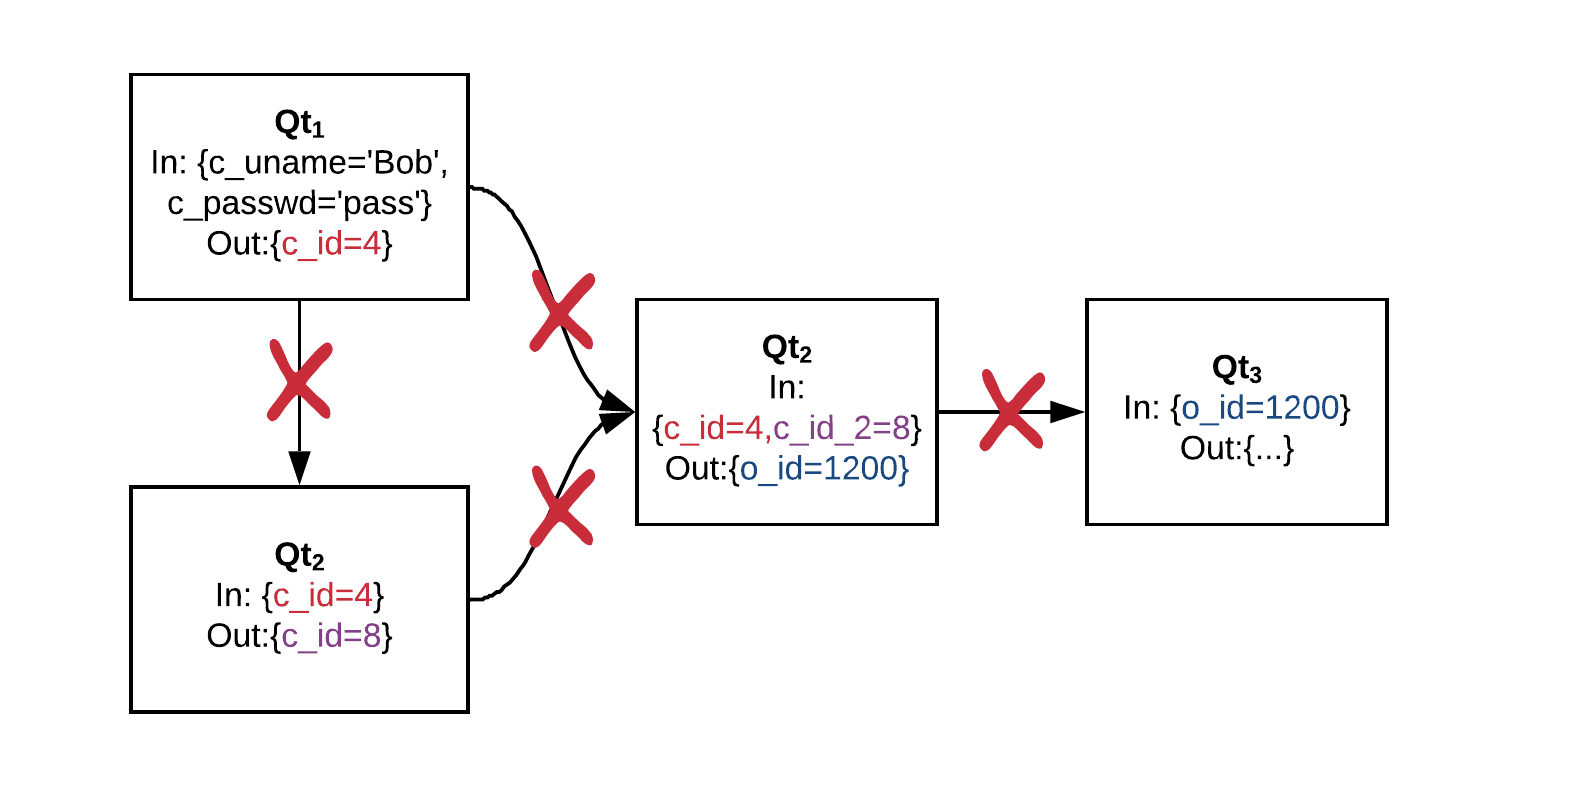
\includegraphics[scale=0.22]{apollo_cpr}
    \end{figure}
\end{frame}

\begin{frame}[fragile]{Predicting Write Queries}
    Although some write queries (INSERT/UPDATE/DELETE) \alert{could} be predicted, incorrect predictive executions of such queries would result
    in modified database state that would need to be undone later.\\

    By predictively executing only read queries, we keep our caching behaviour \alert{strictly complementary}.
\end{frame}



\begin{frame}[fragile]{Always Defined Queries}
    An \alert{always defined query} is a query whose inputs are always satisfied.
\medskip
    \visible<2->{
       The query can be executed and cached at any time!
    }
\end{frame}

\begin{frame}[fragile]{Reloading Always Defined Queries}
Reload an always defined query after executing a write query if:
\begin{itemize}
    \visible<2->{
    \item{The query was invalidated!}
    }
    \visible<3->{
    \item{The query is considered \alert{valuable}: \\
        $likelihood\_of\_query(\mathit{Qt})\cdot avg\_response\_time(\mathit{Qt}) \geq \textrm{reload threshold}$
    }
    }
\end{itemize}
\end{frame}

\section{Apollo}

\begin{frame}[fragile]{Apollo Architecture}
    \begin{figure}
        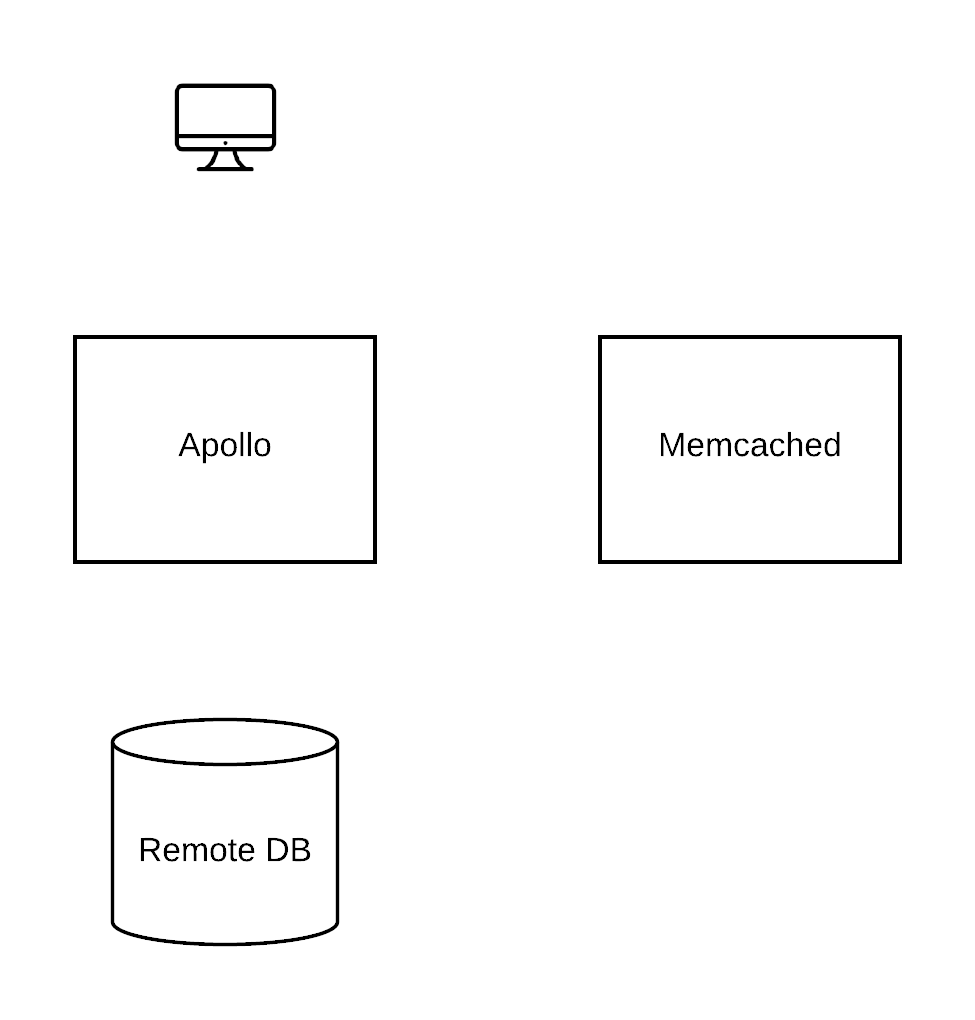
\includegraphics[scale=0.17]{apollo_arch_diagram}
    \end{figure}
\end{frame}

\begin{frame}[fragile]{Apollo Architecture}
    \begin{figure}
        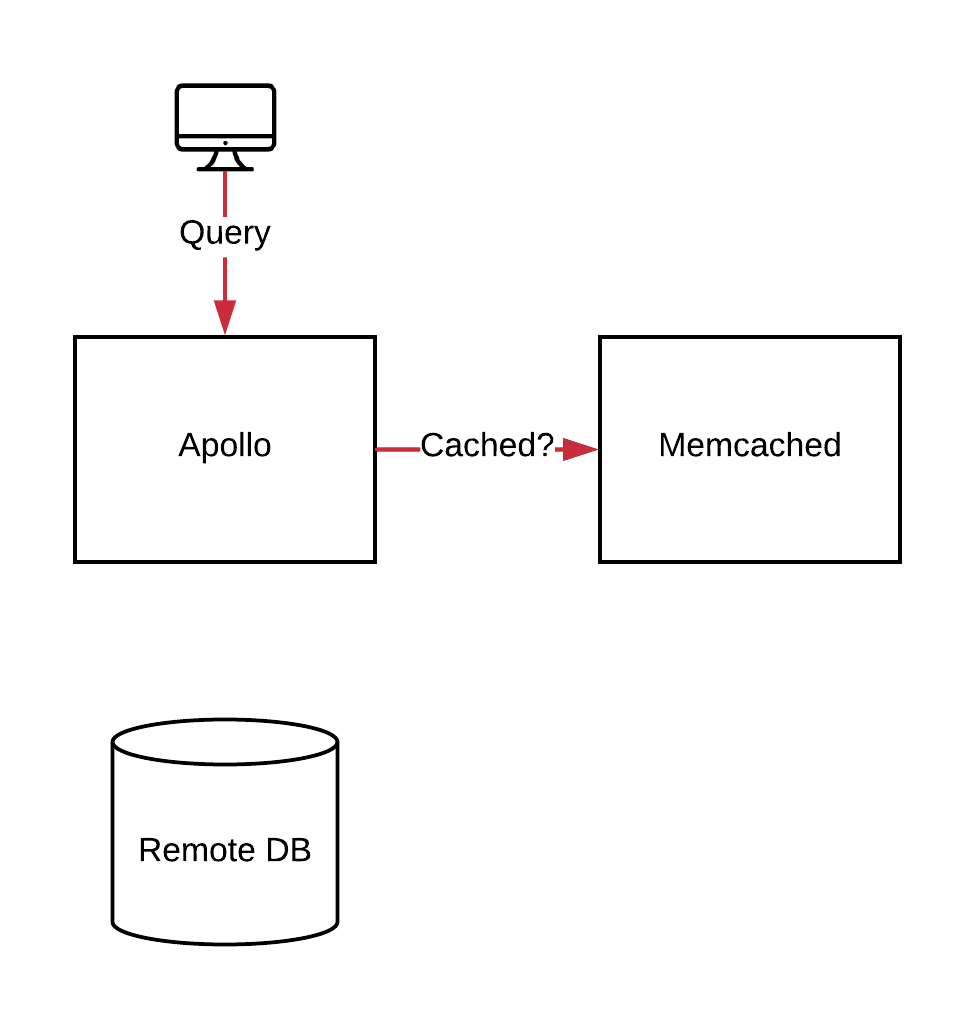
\includegraphics[scale=0.17]{apollo_arch_diagram_2}
    \end{figure}
\end{frame}

\begin{frame}[fragile]{Apollo Architecture}
    \begin{figure}
        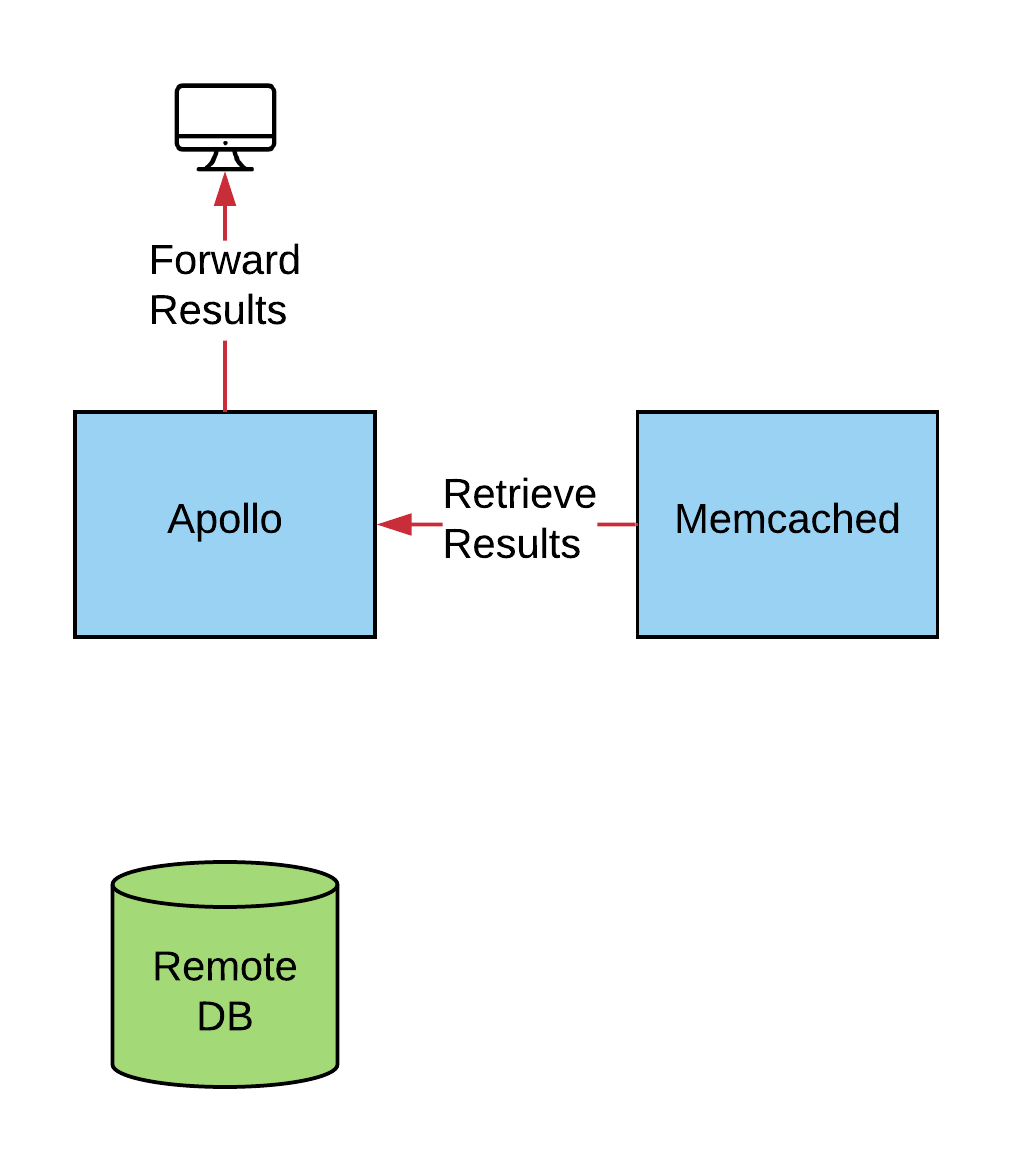
\includegraphics[scale=0.17]{apollo_arch_diagram_3}
    \end{figure}
\end{frame}

\begin{frame}[fragile]{Apollo Architecture}
    \begin{figure}
        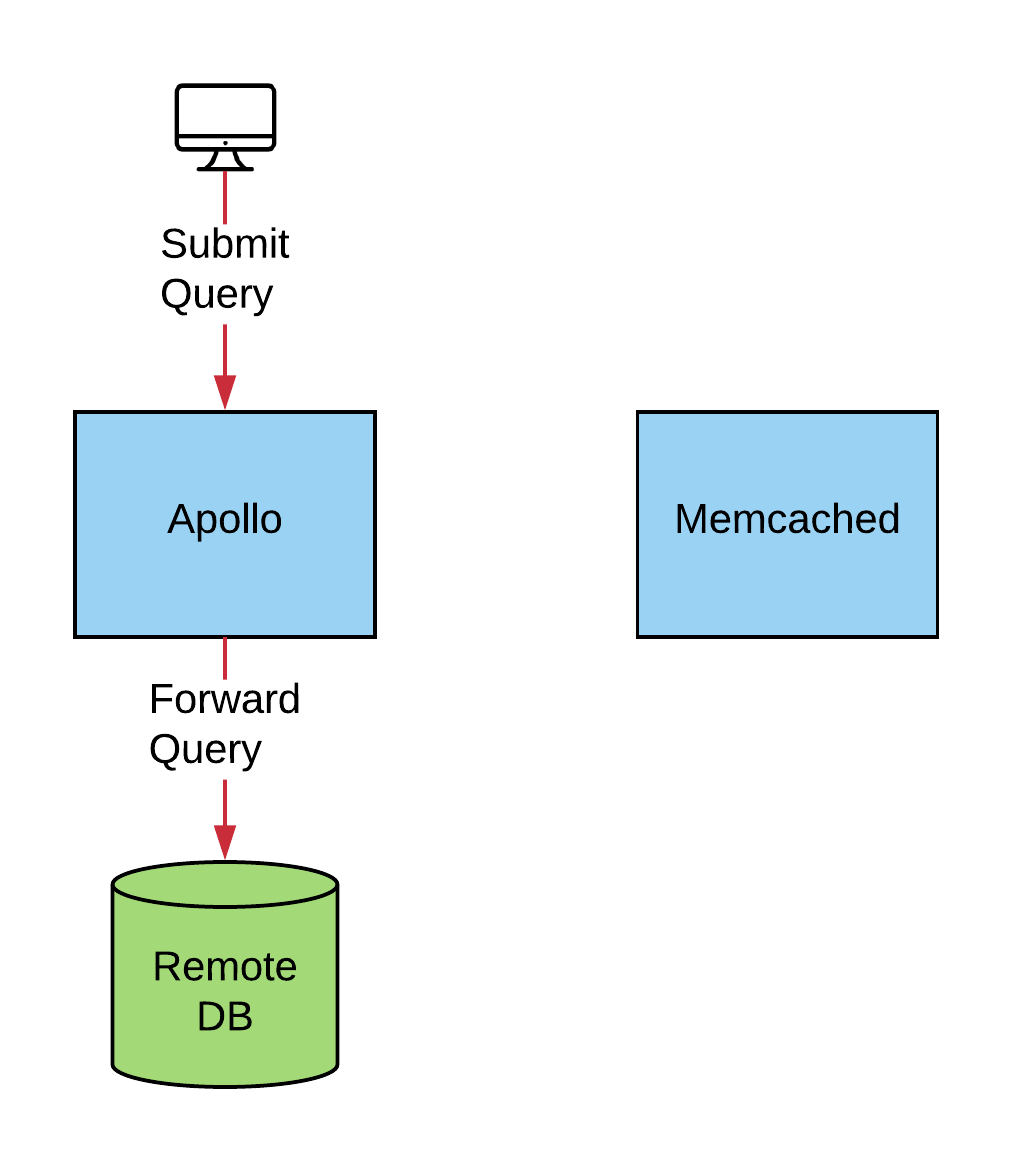
\includegraphics[scale=0.17]{apollo_arch_diagram_4}
    \end{figure}
\end{frame}

\begin{frame}[fragile]{Apollo Architecture}
    \begin{figure}
        \includegraphics[scale=0.17]{apollo_arch_diagram_6}
    \end{figure}
\end{frame}

\begin{frame}[fragile]{Apollo Architecture}
    \begin{figure}
        \includegraphics[scale=0.17]{apollo_arch_diagram_7}
    \end{figure}
\end{frame}

\begin{frame}[fragile]{Apollo Architecture}
    \begin{figure}
        \includegraphics[scale=0.17]{apollo_arch_diagram_8}
    \end{figure}
\end{frame}

\begin{frame}[fragile]{Publish---Subscribe Model}
Concurrent requests proxied to the remote DB or memcached for the same read-query will be blocked until the original query has returned.
That query's result set will be \alert{forwarded} to the others.
\end{frame}

\begin{frame}[fragile]{Client Sessions}
Clients are guaranteed to see state at least as recent as what they last read/wrote.
    \begin{itemize}
    \visible<2->{
    \item{\alert{Client-centric} approach to caching!}
    }
    \visible<3->{
    \item{\alert{Writes} and \alert{``future reads''} update client version and cause invalidations.}
    }
    \end{itemize}
\end{frame}

\begin{frame}{Benefits}
    \begin{figure}
        \center
        \hspace*{-1.5cm}
        \includegraphics[scale=0.17]{apollo_ec_upd}
    \end{figure}
\end{frame}

\begin{frame}[fragile]{Benefits}
    \begin{itemize}
        \item{No global cache invalidations.}
        \item{Can predict whether a prefetched query result will be used before invalidation!}
    \end{itemize}
\end{frame}

\begin{frame}[fragile]{Prediction Invalidation Detection}
    \begin{figure}
        \includegraphics[scale=0.22]{apollo_query_pipeline}
    \end{figure}
\end{frame}

\begin{frame}[fragile]{Prediction Invalidation Detection}
    \begin{figure}
        \center
        \includegraphics[scale=0.22]{apollo_write_boundary}
    \end{figure}
\end{frame}

\begin{frame}[fragile]{Prediction Invalidation Detection}
    \begin{figure}
        \center
        \includegraphics[scale=0.22]{apollo_write_boundary_2}
    \end{figure}
\end{frame}

\begin{frame}[fragile]{Prediction Invalidation Caching}
    \begin{itemize}
    \visible<2->{
    \item{Maintain multiple client query graphs with different $\Delta t$ widths}
    \item{Consult client query graphs to see if a query is likely to occur that would invalidate the results of our predictively executed query}
    }
    \end{itemize}
\end{frame}

\begin{comment}
\begin{frame}[fragile]{Example}
    \alert{Problem:}\\
    Result set from client submitted $\mathit{Qt}_1$ just came back. We have complete mappings from $\mathit{Qt}_1$ to
    $\mathit{Qt}_2$ and from $\mathit{Qt}_2$ to $\mathit{Qt}_3$. Each query template takes an average of $t=2$ to execute. Do we execute $\mathit{Qt}_2$?
    Do we execute $\mathit{Qt}_3$?
\end{frame}

\begin{frame}[fragile]{Do we execute $\mathit{Qt}_2$?}
    $\mathit{Qt}_2$ is estimated to take $t=2$ to execute.
    \visible<2>{
        \begin{figure}
            \center
            \includegraphics[scale=0.17]{apollo_session_aware_caching}
        \end{figure}
    }
\end{frame}

\begin{frame}[fragile]{Do we execute $\mathit{Qt}_2$?}
    $\mathit{Qt}_2$ is estimated to take $t=2$ to execute.
    \begin{figure}
        \center
        \includegraphics[scale=0.17]{apollo_session_aware_caching_2}
    \end{figure}
\end{frame}

\begin{frame}[fragile]{Follow out-arrows from $\mathit{Qt}_1$}
    \begin{figure}
        \center
        \includegraphics[scale=0.3]{apollo_session_aware_caching_3}
    \end{figure}
\end{frame}

\begin{frame}[fragile]{Follow out-arrows from $\mathit{Qt}_1$}
    \begin{figure}
        \center
        \includegraphics[scale=0.3]{apollo_session_aware_caching_4}
    \end{figure}
    \visible<2->{
        $\mathit{Qt}_2$ is likely ($P(\mathit{Qt}_2|\mathit{Qt}_1;T\leq 2)=1.0$) to show up within $t=2$.\\
        No queries predicted to invalidate the $\mathit{Qt}_2$'s result set, so execute it and cache it.
    }
\end{frame}

\begin{frame}[fragile]{What about $\mathit{Qt}_3$?}
    \begin{figure}
        \includegraphics[scale=0.22]{apollo_query_pipeline}
    \end{figure}
    After $\mathit{Qt}_2$ has executed, should we execute $\mathit{Qt}_3$? \\
    \visible<2->{
        $\mathit{Qt}_3$ is estimated to take $t=2$ to execute.\\
    }
\end{frame}

\begin{frame}[fragile]{Do we execute $\mathit{Qt}_2$?}
    $\mathit{Qt}_3$ is estimated to take $t=2$ to execute.
    \begin{figure}
        \center
        \includegraphics[scale=0.17]{apollo_session_aware_caching_2}
    \end{figure}
\end{frame}

\begin{frame}[fragile]{Follow out-arrows from $\mathit{Qt}_2$}
    \begin{figure}
        \center
        \includegraphics[scale=0.27]{apollo_session_aware_caching_3}
    \end{figure}
\end{frame}

\begin{frame}[fragile]{Follow out-arrows from $\mathit{Qt}_2$}
    \begin{figure}
        \center
        \includegraphics[scale=0.27]{apollo_session_aware_caching_5}
    \end{figure}
    \visible<2->{
        $\mathit{Qt}_w$ is likely ($P(\mathit{Qt}_w|\mathit{Qt}_2;T\leq 2)=0.75$) to show up within $t=2$.\\
        $\mathit{Qt}_w$ will increase the client's session, so predictively executing $\mathit{Qt}_3$ is unlikely to be useful.
    }
\end{frame}
\end{comment}

\section{Experiments}

\begin{frame}[fragile]{Experiment Configuration}
    \begin{figure}
        \center
        \includegraphics[scale=0.17]{apollo_exp_config}
    \end{figure}
\end{frame}

\begin{frame}[fragile]{Experiment Configuration}
    Three configurations:
    \begin{itemize}
        \item{\alert{Apollo configuration:} as described in prior sections.}
        \item{\alert{Memcached configuration:} LRU cache --- Apollo with predictive features turned off}
        \item{\alert{Fido configuration:} Use Fido predictive engine instead of Apollo's predictive features!}
    \end{itemize}
\end{frame}

\begin{frame}[fragile]{Fido}
    \begin{itemize}
        \item{Query instance based predictions, instead of query templates.}
            \begin{itemize}
                \item{$Q_1, Q_2, Q_3$ in query stream.}
                \item{Look for previous execution of queries prefixed by those: (i.e. $Q_1, Q_2, Q_3, Q_4, Q_5$), execute up to 10 predictions}
                \item{Prefix length: 3, Suffix Length: 2}
            \end{itemize}
        \item{Requires offline training.}
    \end{itemize}
\end{frame}

\begin{frame}[fragile]{TPC-W Results}
    \begin{figure}
        \center
        \includegraphics[scale=0.7]{apollo_tpcw}
    \end{figure}
\end{frame}

\begin{frame}[fragile]{Learning Over Time}
    \begin{figure}
        \center
        \includegraphics[scale=0.7]{apollo_30_intervals}
    \end{figure}
\end{frame}

\begin{frame}[fragile]{Workload Change}
    \begin{figure}
        \center
        \includegraphics[scale=0.11]{apollo_wl_change}
    \end{figure}
\end{frame}

\begin{frame}[fragile]{Multiple Apollo Instances}
    \begin{figure}
        \center
        \includegraphics[scale=0.7]{apollo_scalability_curve}
    \end{figure}
\end{frame}

\begin{frame}[allowframebreaks]
    \bibliographystyle{abbrv}
    \bibliography{demo}
\end{frame}


\end{document}
